\documentclass{article}

\usepackage{ctex}
\usepackage{tikz}
\usetikzlibrary{automata, positioning, arrows}
\usetikzlibrary{cd}

\usepackage{amsthm}
\usepackage{amsmath}
\usepackage{amssymb}
%\usepackage{stmaryrd}
\usepackage{mathtools}
\usepackage{proof}

\usepackage[linesnumbered,ruled,vlined]{algorithm2e}

\usepackage[cache=false]{minted} %code block

%\usepackage{unicode-math}
\PassOptionsToPackage{hyphens}{url}\usepackage{hyperref} %url解决过长的问题
\usepackage{hyperref} %url
\hypersetup{
    colorlinks=true,
    linkcolor=blue,
    filecolor=magenta,      
    urlcolor=cyan,
    pdftitle={Overleaf Example},
    pdfpagemode=FullScreen,
    }


\usepackage[textwidth=18cm]{geometry} % 设置页宽=18

\usepackage{blindtext}
\usepackage{bm}
\parindent=0pt
\setlength{\parindent}{2em} 
\usepackage{indentfirst}

\usepackage{xcolor}
\usepackage{titlesec}
\titleformat{\section}[block]{\color{blue}\Large\bfseries\filcenter}{}{1em}{}
\titleformat{\subsection}[hang]{\color{red}\Large\bfseries}{}{0em}{}
%\setcounter{secnumdepth}{1} %section 序号

\newtheorem{theorem}{Theorem}[section]
\newtheorem{lemma}[theorem]{Lemma}
\newtheorem{corollary}[theorem]{Corollary}
\newtheorem{proposition}[theorem]{Proposition}
\newtheorem{example}[theorem]{Example}
\newtheorem{definition}[theorem]{Definition}
\newtheorem{remark}[theorem]{Remark}
\newtheorem{exercise}{Exercise}[section]
\newtheorem{annotation}[theorem]{Annotation}


%{\mathlarger{\mathlarger\mathlarger{\mathlarger{\oldPi}}}}

\newcommand\Set[2]{\{\,#1\mid#2\,\}} %集合
\newcommand\SET[2]{\Set{#1}{\text{#2}}} %

\newcommand{\redt}[1]{\textcolor{red}{#1}}
\newcommand{\bluet}[1]{\textcolor{blue}{#1}}
\newcommand{\abracket}[1]{\ensuremath{\left< #1 \right>}}

\newcommand*{\xfunc}[4]{{#2}\colon{#3}{#1}{#4}}
\newcommand*{\func}[3]{\xfunc{\to}{#1}{#2}{#3}}


\newcommand{\inl}[1]{\ensuremath{\text{inl}~#1}}
\newcommand{\inr}[1]{\ensuremath{\text{inr}~#1}}
\newcommand{\fold}[1]{\ensuremath{{fold}_{#1}}}
\newcommand{\unfold}[1]{\ensuremath{{unfold}_{#1}}}
\newcommand{\lam}[2]{\ensuremath{\lambda #1\ldotp #2}} %lamx.y
\newcommand{\pair}[1]{\ensuremath{\left\langle#1\right\rangle}}
\newcommand{\projone}[1]{\ensuremath{#1.1}}
\newcommand{\projtwo}[1]{\ensuremath{#1.2}}
\newcommand{\caseof}[3]{\ensuremath{{\textbf{case}}~#1~{\textbf{of}}~\inl{x_1}\mapsto #2\mid\inr{x_2}\mapsto #3}}
\newcommand{\Lam}[2]{\ensuremath{\Lambda #1\ldotp #2}}
\newcommand{\pack}[3]{\ensuremath{{pack}~\pair{#1,#2}~{as}~#3}}
\newcommand{\unpack}[4]{\ensuremath{{unpack}~#1~{as}~\pair{#2,#3}~{in}~#4}}
\newcommand{\assign}[2]{\ensuremath{#1~\coloneqq~#2}}
\newcommand{\singletype}[1]{\text{#1}}
\newcommand{\termtype}[2]{\ensuremath{#1:#2}}
\newcommand{\type}[3]{\ensuremath{ \left\{#1:#2\relmiddle|#3 \right\}}}
\newcommand{\matgen}[2]{\ensuremath{\mu #1\ldotp#2}} %ux.y
\newcommand{\mat}[0]{\matgen{\alpha}{\tau}} %ua.t
\newcommand{\fatgen}[2]{\ensuremath{\forall #1\ldotp#2}}
\newcommand{\fat}[0]{\fatgen{\alpha}{\tau}}
\newcommand{\eatgen}[2]{\ensuremath{\exists #1\ldotp#2}}
\newcommand{\eat}[0]{\eatgen{\alpha}{\tau}}
\newcommand{\fatgent}[2]{\ensuremath{\trgb{\forall} #1\ldotp#2}}
\newcommand{\fatt}[0]{\fatgent{\alpt}{\tat}}
\newcommand{\eatgent}[2]{\ensuremath{\trgb{\exists} #1\ldotp#2}}
\newcommand{\eatt}[0]{\eatgent{\alpt}{\tat}}

\newcommand{\fail}[0]{\mi{fail}}

\newcommand{\bnfdef}[0]{\ensuremath{\mathrel{::=}}} %::=
\newcommand{\term}[1]{\ensuremath\mathsf{#1}}
\newcommand{\true}{\term{true}}
\newcommand{\false}{\term{false}}
\newcommand{\ifelse}[3]{\ensuremath{\textbf{if}~#1~\textbf{then}~#2~\textbf{else}~#3}}
\newcommand{\newwhiledo}[2]{\ensuremath{\textbf{while}~#1~\textbf{do}~#2}}
\newcommand{\letvar}[2]{\ensuremath{\textbf{letvar}~#1~\textbf{in}~#2}}
\newcommand{\succt}[1]{\term{succ}~#1}
\newcommand{\pred}[1]{\term{pred}~#1}
\newcommand{\iszero}[1]{\term{iszero}~#1}
\newcommand{\seq}[2]{#1;#2}
\newcommand{\subtyp}[2]{#1<:#2}

\newcommand{\dbracket}[1]{\ensuremath{\left\llbracket\,\vcenter{\hbox{$#1$}}\,\right\rrbracket}}

\newcommand{\todo}[1]{\textcolor{red}{TODO: #1}\PackageWarning{TODO:}{#1!}}

\newcommand{\defeqv}{\vcentcolon\equiv}
\newcommand{\refl}{\textbf{refl}}
\newcommand{\id}{\textbf{id}}
\newcommand{\ind}{\textbf{ind}}
\newcommand{\ap}{\textbf{ap}}
\newcommand{\apd}{\textbf{apd}}
\newcommand{\transport}{\textbf{transport}}
\newcommand{\transportconst}{\textbf{transportconst}}
\newcommand{\lift}{\textbf{lift}}
\newcommand{\pr}{\textbf{pr}}
\newcommand{\qinv}{\textbf{qinv}}


%variable name
\ExplSyntaxOn 
\NewDocumentCommand{\vn}{m}
 {
   \seq_set_split:Nnn \l_tmpa_seq { ~ } { #1 }
   \int_compare:nTF { \seq_count:N \l_tmpa_seq > 1 }
    {
     \seq_set_map:NNn \l_tmpb_seq \l_tmpa_seq { \exp_not:N \mathit { ##1 } }
     (\seq_use:Nn \l_tmpb_seq { \  })
    }
    { \mathop{}\!\mathit{#1} }
 }
\ExplSyntaxOff


\begin{document}
\title{关于Maple Algebra的这一路}
\author{枫聆 (maplegra)}
\maketitle
\tableofcontents
\newpage

\section{Logic}

\subsection{Classic Logic}

\begin{annotation}
\rm Double negation和excluded middle是logical equivalent, 关于它们有两个通俗解释:
\begin{itemize}
	\item Double negation: 如果你想证明$P$为$true$, 只需要说明$P$不是$false$即可.
	\item Excluded middle: 任意一个命题$P$, 它不是$true$就是$false$.
\end{itemize}
\end{annotation}

\subsection{Higher-order logic}

\begin{annotation}
\rm Second-order logic在first-order logic的基础上,给其中的谓词也加上了量词. 给谓词加量词意义是什么呢? 谓词实际上可以理解为varibles的properties,所以相当于你给variable's properties也加上了量词. 形如:
\[
	\exists P.\ P(b)
\]
这里的$P$可以看做一个谓词变量(predicate variable). 从语义上来说$P$可以理解为集合,更进一步说就是满足某种property的varibles组成的set, 所以你对$P$施加一个量词也就是在考虑不同的集合,此时上面的formula可以非正式地理解为存在某个集合$P$包含$b$.
\end{annotation}

\subsection{Quantifier Elimination}

\begin{annotation}
\rm Fourier-Motzkin algorithm适用于prenex form下内部formula是一个conjunction且里面的每个conjuncts只能是一个literals i.e., $\forall {x_1,x_2,\cdots,x_n}.~ x_1 > a_1 \wedge x_2 > a_2 \wedge \cdots \wedge x_n > a_n$. 我们将这个算法记为$\pi$, 那么只要我们把任意的formula都转换称DNF,
\end{annotation}

\begin{annotation}
\rm David Monniaux (CAV'10)中提到可以利用SMT-solver来把任意quantifer-free formula转换成DNF, 这样我们对其中DNF中的每一个clause都可以分开来使用Fourier-Motzkin algorithm. 它具体的做法就是,对于给定的formula $F$, 扔给SAT-solver, 如果是satisfiable的,那么SAT-solver就会给出一个solution, 这个solution实际对应一个conjunction $C$ (由$F$中atoms构造的,如果solution某个variable使得对应的atom是true, 那么就把这个atom丢到conjunction中,反之把negation of atom丢到conjunction中)使得$C \rightarrow F$. 这样我们再把$F \wedge \neg C$扔到SMT-solver中,类似一直操作,直到unsat. 

这种方式存在一个问题, 如果给定$F \equiv (x_1 = 0 \vee x_1 = 1) \wedge \cdots \wedge (x_n = 0 \vee x_n = 1)$, 那么将产生$2^n$个conjuncts. 而对于$\exists x_2,\cdots,x_n.~F$, 它的quantifier free形式却只是$x_1 = 0 \vee x_1 = 1$ (logically equivalent quantifier-free formula). 显然有点不太efficient,这个时候我们不直接用$F \wedge C$, 而用$F \wedge \neg \pi(\exists x_2,\cdots,x_n.~C)$作为新一轮的查询. 例如这里设$C \equiv (x_1 = 0 \wedge x_2 = 0 \wedge \cdots \wedge x_n = 0)$, 那么$\pi(C) \equiv x_1 = 0$, 这样我们只需要call SAT-solver两次就可以得到我们想要的DNF. 

David Monniaux提出的优化方法远不止于此,其核心在于对nested quantifiers如何处理. 如果此时给定$F \equiv \exists x.\forall y.\exists z. ~ z \geq 0 \wedge ((x \geq z \wedge y \geq z) \vee y \leq 1 - z)$, 显然这个$F$是valid的. 我们从内向外一层层去掉quantifiers.
\begin{itemize}
    \item 设最里面的quantifier-free formula为$F_3$, 它并不是DNF, 尝试转化为DNF. 假设扔给SMT-solver得到solution $x = 0 \wedge y =0 \wedge z = 0$, 对应的conjunction为$C_1 \equiv z \geq 0 \wedge x \geq z \wedge y \geq z \wedge y \leq 1 - z$, 那么$\pi(\exists z.~C_1) \equiv x \geq 0 \wedge y \geq 0 \wedge y \leq 1$. 再把$F_3 \wedge \neg \pi(C)$丢到SMT-solver中得到solution $x = 0 \wedge y = -1 \wedge z = 2$, 对应的conjunction为$C_2 \equiv z \geq 0 \wedge x \geq z \wedge y \leq 1 - z$, 那么$\pi(\exists z.~C_2) \equiv x \geq 0 \wedge y \leq 1$. 如此继续,设$F_2 \equiv \exists z. F_3$, 最后有$F_2 \equiv \bigvee \pi(\exists z.~C_i) \equiv x \geq 0 \vee y \leq 1$. 
    \item 设$F_1 = \forall y.~F_2$, 那么显然有$F_1 \equiv x \geq 0$.
    \item 最后$\exists x. F_1 \equiv true$.
\end{itemize}
注意到如果我们只取quantifier-free $F_2$中的conjunct $x \geq 0$, 使得$F_2' \equiv x \geq 0$, 对$\exists x.\forall y. ~F_2'$做quantifier elimination,最后也能得到$true$这个结果. 这意味着我们不用在最里面那个阶段费尽心思地构造完整的DNF. 也就是说用“比较强的formula”得到了一个结果,那么显然“弱一点的formula”也是有这个结果的. 但是只有当这个结果是true的时候,这么做才有意义,不然出现false的时候,你并不能说明它是false的, 其他情况给不出原formula准确的quantifier-free form.

我还是想记录这个算法的全过程推理,因为花了不少精力,将来忘记了就比较可惜. 算法如图\ref{fig:qe-sat}, 其每个关键的步骤细节如下:
\begin{itemize}
    \item 首先是关于这里$F_0, F_1, \cdots F_n$的定义: $F_0$是一个形如$\forall_{B_0}\exists_{B_1}\forall_{B_2}\cdots F$的prenex. 其中$B_0,B_1,B_2,\cdots$就是把相邻地相同的quantifiers合起来. 对于任意$i \geq 0$, $F_i = \forall \neg F_{i+1}$, 注意这里是从$F_0$往后构造$F_i$的. 例如给定$\forall x. \exists y.\forall z~G$, 它对应的$F_i$分别为
    \[
        \begin{tabular}{l}
        $F_0 = \forall x. \exists y.\forall z~G$ \\
        $F_1 = \forall y. \exists z.~\neg G$ \\
        $F_2 = \forall z.~G$ \\
        $F_3 = \neg G$
        \end{tabular}
    \]
    \item 这里$\textsc{SMT-Test}(C, F)$用于判断$C \wedge F$是否是satisfiable,它的返回值为$(b, C')$, 其中$b$是一个boolean value表示是否satisfiable. 当$b = true$时,有$\text{atoms}(C') \subseteq \text{atoms}(F)$, 且满足$C' \Rightarrow F$ and $C \wedge C'$ is satisfiable. 这一点很容易办到,参考上面由solution生成对应conjunction的过程; 当$b=false$时,$C = false$.
    \item 其中$M_0,M_1,\cdots,M_{n-1}$初始化为$true$, 满足对任意的$i < n$有$F_i \Rightarrow M_i$. 注意在$\textsc{Q-Test}$的每一步都会保持这个条件.
    \item 最关键的$\textsc{Q-Test}(i, C)$, 设它的返回值为$(b, C')$, 其中$b$表示$F_i \wedge C$表示是否satisfiable. \redt{(性质1)如果$b = true$, 有$\text{FV}(C) = \text{FV}(F_i)$, 且满足$C' \Rightarrow F_i$ and $C \wedge C'$ is sat}. 那这个算法和quantifier elimination有什么关系呢? 考虑$\textsc{Q-Test}(0, true)$, 当它第一个返回值为$true$的时候,就有$C' \Rightarrow F_0$, 并且$C'$是quantifier-free的. 这个时候我们就得到了一个比如强的formula $C'$, 拿它可以进一步去测试$\forall F_0$或者$\exists F_0$就有意义了. 最大的缺点是给不出准确原完整的quantifier-free form. 也就是我们无法保证$F_0 \Rightarrow C'$.
    
    %恰好地是算法本身返回时, 也会保持一个额外的\redt{(性质2), 当$i < n$时有$F_i \wedge C \Rightarrow C'$}. 当包含量词的时候总有$n \geq 1$. 这就意味当$i = 0$时,有$F_0 \Rightarrow C'$. 所以整个算法的correctness是Ok的.  
    
    前面我们把算法基本核心描述了一下, 我们下面一步一步来看:
    \begin{itemize}
        \item 当$i = n$, 如果$F_n \wedge C$ is unsat, 那么$F_n \wedge C \Rightarrow false$且$false \Rightarrow F_n$, 即返回值$(false, false)$. 如果$F_n \wedge C$ is sat, $C' \Rightarrow F_n$是显然的,还对$C'$做了一次泛化(generalization)找到弱一点$C''$依然符合条件. 因为我们希望最终得到的那个强的formula能更弱一点,尽量贴近$F_n$. 
        \item 当$i < n$时,看下面这个while循环. 当$b' = false$时,由$C \wedge M_i$ is unsat可以马上得到$C \wedge F_i$ is unsat, 因为$F_i \Rightarrow M_i$ (在后面唯一修改$M_i$的地方,我们会证明这个关系在$M_i$被修改之后依然保持). 因此$\textsc{Q-Test}(i, C)$返回$(false, false)$, 性质1是显然保持的.
        
        当$b' = true$时,此时由$C \wedge M_i$ is sat还不能确定$C \wedge F_i$ is sat. 同时是否有$C' \Rightarrow  F_i$也不能确定,想确定它可以按照下面思路
        \[
            \begin{tabular}{l}
                $C' \Rightarrow  F_i$ is valid \\
                $\equiv \neg (C' \Rightarrow F_i)$ is unsat \\
                $\equiv C' \wedge \neg F_i$ is unsat \\
                $\equiv C' \wedge \exists_{B_i} F_{i+1}$ is unsat (by $F_i = \forall_{B_i} \neg F_{i+1}$)\\
            \end{tabular}
        \]
        这里有$FV(C') \subseteq FV(\exists_{B_i} F_{i+1})$, 那么这里最后只需要确定$C' \wedge F_{i+1}$是否是unsat的,直接调用$\textsc{Q-Test}(i+1, C')$即可. 如果其返回值$b'' = false$, 直接返回经过前面的分析是满足性质1的. 这里也还做一下generalization, 也是希望最终得到的那个强的formula能更弱一点, 尽量贴近$F_i$. 
        
        如果其返回值$b'' = true$, 那么我们不能确定$C' \Rightarrow F_i$. 但是我们得到了一个$C''$使得$C'' \Rightarrow F_{i+1}$ and $C' \wedge C''$ is satisfiable. 就是这个$C''$ 使得$C' \wedge \exists_{B_i} F_{i+1}$ is sat, 如果我们未来想得到一个新的$C'$满足$C' \Rightarrow F_i$, 就要尽量把$C''$排除出去. 因此把$\neg \pi(\exists_{B_i} C'')$加到$M_i$中. 这里我们需要确认一下$F_i \Rightarrow M_i$是否依然保持. 由于$C'' \Rightarrow F_{i+1}$, 所以有$\exists_{B_i} C'' \Rightarrow \exists_{B_i} F_{i+1}$, 它的逆否命题为$\forall_{B_i} \neg F_{i+1} \to \neg \exists_{B_i} C''$, 其左边是等价于$F_i$, 右边等价于$\neg \pi(\exists_{B_i} C'')$.
    \end{itemize}
\end{itemize}
\begin{figure}[H]
    \centering
    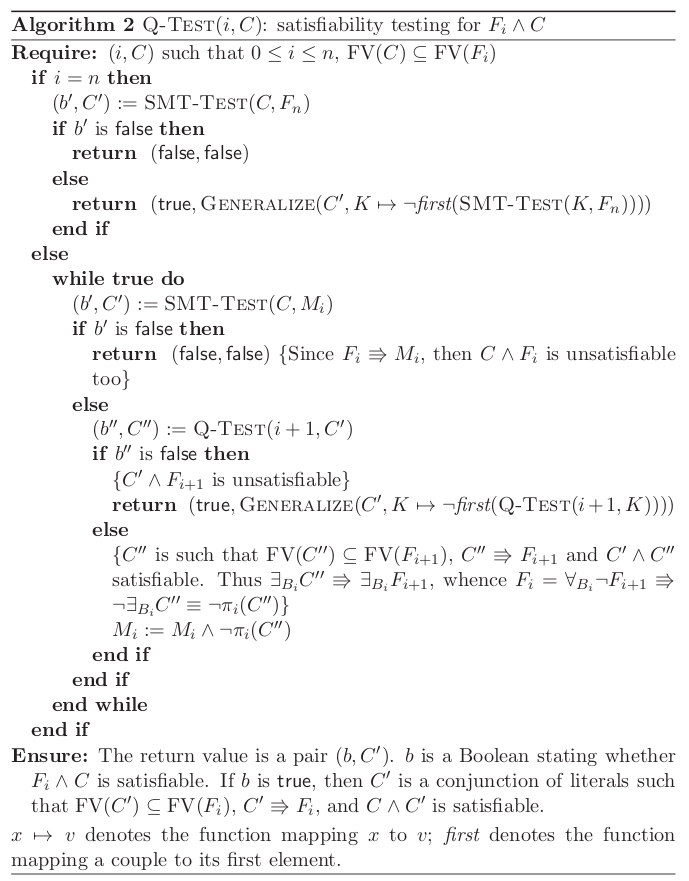
\includegraphics[width=0.8\textwidth]{images/qe-sat.png}
    \caption{Q-Test}
    \label{fig:qe-sat}
\end{figure}
\end{annotation}

\newpage
\subsection{Misc}

\begin{definition}
\rm A set of logical connectives is called \redt{functionally complete} if every boolean expression is equivalent to one involving only these connectives.
\end{definition}

\begin{definition}
\rm 简而言之,如果任意的logical formula都可以只用给定的一些logical connectives来构造一个等价的新的logical formula, 我们就说这些这些logical connectives组成的system是functionally complete. 
\end{definition}

\begin{example}
\rm 列举一些在classic logic下functionally complete的system:
\begin{itemize}
	\item $\{\downarrow\}$, $\{\uparrow\}$, 其中$\downarrow$表示$A \downarrow B = \neg (A \vee B)$, $\uparrow$表示$A \uparrow B = \neg (A \wedge B)$.
	\item $\{\vee ,\neg \}$, $\{\wedge ,\neg \}$, etc.
	\item $\{\land ,\lor ,\rightarrow \}$, etc.
\end{itemize}
\end{example}

\section{Language}

\subsection{Standard Semantics}

\begin{annotation}
\rm Operational semantics关注给定一个initial state会得到怎样的final state, 每一个CFG's node对应一个transfer function $f:\mathcal{S} \to \mathcal{S}$
\[
	\lam{s}{(\mu(s),next)}.
\]
其中$f$表示对state $s$的update, next表示下一个将要进入的node. 那么operational semantics的一个解释过程可以用递归的形式定义:
\[
	\vn{interp} = \lam{s}{\lam{n}{\ifelse{isExitNode(n)}{s}{\mathbf{let}~(s',n')=f_n(s)~\mathbf{in}~\vn{interp}~s'~n'}}}
\]
如果我们希望得到一个准确的定义,即不希望等式两边都包含$\vn{interp}$,那么我可以利用一个trick
\[
\vn{semantics} = \vn{fix}(\lam{F}{\lam{s}{\lam{n}{\ifelse{isExitNode(n)}{s}{\mathbf{let}~(s',n')=f_n(s)~\mathbf{in}~F~s'~n'}}}})
\]
你仔细观察一下这个fixpoint就是$\vn{interp}$本身.
\end{annotation}

\subsection{Collecting Semantics}

\begin{annotation}
\rm Collecting semantics和operational semantics不同的是,每一个CFG's node可能对应了一个set of states, 而不是单一的state了. 因为collecting semantics从一开始就把所有可能的initial states作为了一个set来考虑. 因此此时的transfer function为$f:\mathcal{P}(\mathcal{S}) \to \mathcal{P}(\mathcal{S})$:
\[
f_{n \to m} = \lam{S}{\Set{s'}{s \in S ~\text{and}~f_n(s)=(s',m)}}
\]
\end{annotation}

\subsection{Language equation and Arden's Rule}

\begin{theorem}
\rm The set $A^* \cdot B$ is the smallest language that is a solution for $X$ in the linear equation 
\[
	X = A \cdot X + B
\]
where $X, A, B$ are sets of string and $+$ stands for union of languages. Moreover, If the set $A$ does not contain the empty word, then the solution is unique.
\end{theorem}

\begin{annotation}
\rm \bluet{Arden's rule can be used to help convert some finite automatons to regular expressions}.
\end{annotation}



\newpage
\section{Equivalence of Program}

\subsection{Graph Ismorphism}

\subsection{Accepted Language Equivalentce}

\begin{annotation}
\rm \cite{CCS} Chapter 1.
\end{annotation}

\subsection{Bisimulation and Observation Equivalence}

\begin{definition}
\rm A labelled transition system (LTS) is a tuple $(S, \Lambda, \to)$ where $S$ is set of states, $\Lambda$ is set of labels, and $\to$ is relation of labelled transitions (i.e., a subset of $S \times \Lambda \times S$).  A $(p,\alpha,q) \in \to$ is written as $p  \xrightarrow{\alpha} q$. 
\end{definition}

\begin{annotation}
\rm \todo{categorical semantics: $F$-coalgebra}
\end{annotation}


\begin{definition}
\rm \cite{ITLTS}Let $T=(S,\Lambda,\to)$ be a labelled transition system. The set of \redt{traces} $\vn{Tr}(s)$, for $s \in S$ is the minimal set satisfying
\begin{itemize}
	\item $\varepsilon \in \vn{Tr}(s)$.
	\item $\alpha~\sigma \in \vn{Tr}(s)$ if $\Set{s' \in S}{s~ \xrightarrow{\alpha}~s' ~\text{and}~\sigma \in \vn{Tr}(s')}$. 
\end{itemize}
\end{definition}

\begin{definition}
\rm Two states $p,q$ are trace equivalent iff $\vn{Tr}(p) = \vn{Tr}(q)$.
\end{definition}

\begin{definition}
\rm (\redt{Simultation}) Given two labelled transition system $(S_1, \Lambda, \to_1)$ and $(S_2, \Lambda, \to_2)$, relation $R \subseteq S_1 \times S_2$ is a simulation iff, for all $(p,q) \in R$ and $\alpha \in \lambda$ satisfies
\[
	\text{for any}~p \xrightarrow{\alpha}_1 p', ~\text{then there exists}~ q'~\text{such that}~q \xrightarrow{\alpha}_2 q'~\text{and}~(p',q') \in R 	
\]
\begin{center}
% https://tikzcd.yichuanshen.de/#N4Igdg9gJgpgziAXAbVABwnAlgFyxMJZABgBpiBdUkANwEMAbAVxiRDRAF9T1Nd9CKACzkqtRizZoA5Fx7s+eAkTIBmMfWatEIAI5ze2JYOQj11TZJ27ZnMTCgBzeEVAAzAE4QAtkjIgcCCQARgsJbRAAHUjGNAALOgMQTx8kACZqQKRVMK02aNiEkGoGOgAjGAYABUUBNg8sRzicYpAGLDAIuAh2qCSU30R-LMQMto6IqDo4OIdW2bo+xDAmBgZcqxAAJVbSiura5R0GppbMuiwGNkhO-q9B0ICgxBzx250pmbnqBaWVtY2ER2dk4QA
\begin{tikzcd}
p \arrow[rrrr, "\alpha"] \arrow[ddd, "R"', dashed] &  &  &  & p' \arrow[ddd, "R", dashed] \\
                                                   &  &  &  &                             \\
                                                   &  &  &  &                             \\
q \arrow[rrrr, "\alpha"']                          &  &  &  & q'                         
\end{tikzcd}
\end{center}
\end{definition}

\begin{definition}
\rm We say $q$ simulates $p$ if there exists a simulation $R$ includes $(p,q)$ (i.e., $(p,q) \in R$), written $p < q$.
\end{definition}

%\begin{lemma}
%\rm The simulation is reflexive and transitive. 
%\end{lemma}


\begin{definition}
\rm (\redt{Bisimultation}) Given two labelled transition system $(S_1, \Lambda, \to_1)$ and $(S_2, \Lambda, \to_2)$, relation $R \subseteq S_1 \times S_2$ is a bisimulation iff both $R$ and its converse $\overline{R}$ are simulations, for all $(p,q) \in R$ and $\alpha \in \Lambda$ satisfies
\[
	\begin{gathered}
	\text{for any}~p \xrightarrow{\alpha}_1 p', ~\text{then there exists}~ q'~\text{such that}~q \xrightarrow{\alpha}_2 q'~\text{and}~(p',q') \in R \\
	\text{for any}~q \xrightarrow{\alpha}_2 q', ~\text{then there exists}~ p'~\text{such that}~p \xrightarrow{\alpha}_1 p'~\text{and}~(p',q') \in R
	\end{gathered} 	
\]
\end{definition}

%\begin{definition}
%\rm A binary relation between state transition systems, associating systems that behave in the same way in that one system simulates the other and vice versa.
%\end{definition}

\begin{example}
\rm 一些bisimulation的例子
\begin{center}
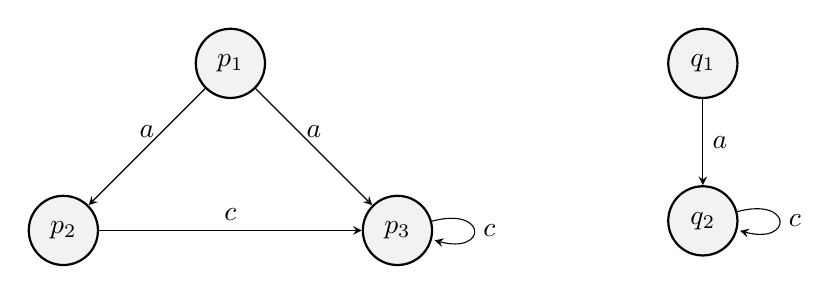
\begin{tikzpicture}
\tikzset{
->, % makes the edges directed
>=stealth, % makes the arrow heads bold
node distance=3cm, % specifies the minimum distance between two nodes. Change if necessary.
every state/.style={thick, fill=gray!10}, % sets the properties for each ’state’ node
initial text=$ $, % sets the text that appears on the start arrow
}
	\node[state] (p1) {$p_1$};
	\node[state, below left of=p1, node distance=3cm] (p2) {$p_2$};
	\node[state, below right of=p1, node distance=3cm] (p3) {$p_3$};
	\node[state, right of=p1, node distance=6cm] (q1) {$q_1$};
	\node[state, below of=q1, node distance=2cm] (q2) {$q_2$};
	
	\draw (p1) edge[above] node{$a$} (p2)
	(p1) edge[above] node{$a$} (p3)
	(p2) edge[above] node{$c$} (p3)
	(p3) edge[loop right] node{$c$} (p3)
	(q1) edge[right] node{$a$} (q2)
	(q2) edge[loop right] node{$c$} (q2);
\end{tikzpicture}
\end{center}
关于上面两个transition system的bisimultaion为$R=\{(p_1,q_1), (p_2,q_2), (p_3,q_2)\}$. 还有一个比较有点特别的例子
\begin{center}
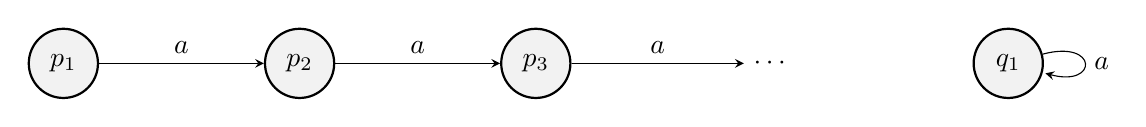
\begin{tikzpicture}
\tikzset{
->, % makes the edges directed
>=stealth, % makes the arrow heads bold
node distance=3cm, % specifies the minimum distance between two nodes. Change if necessary.
every state/.style={thick, fill=gray!10}, % sets the properties for each ’state’ node
initial text=$ $, % sets the text that appears on the start arrow
}
	\node[state] (p1) {$p_1$};
	\node[state, right of=p1, node distance=3cm] (p2) {$p_2$};
	\node[state, right of=p2, node distance=3cm] (p3) {$p_3$};
	\node[right of=p3, node distance=3cm] (p4) {$\cdots$};
	\node[state, right of=p4, node distance=3cm] (q1) {$q_1$};
	
	\draw (p1) edge[above] node{$a$} (p2)
	(p2) edge[above] node{$a$} (p3)
	(p3) edge[above] node{$a$} (p4)
	(q1) edge[loop right] node{$a$} (q1);
\end{tikzpicture}
\end{center}
如果关于上图这样bisimulation $R$存在,那么$(p_i,q_1) \in R$ for every $i$. 再看一个不是bisimulation的例子
\begin{center}
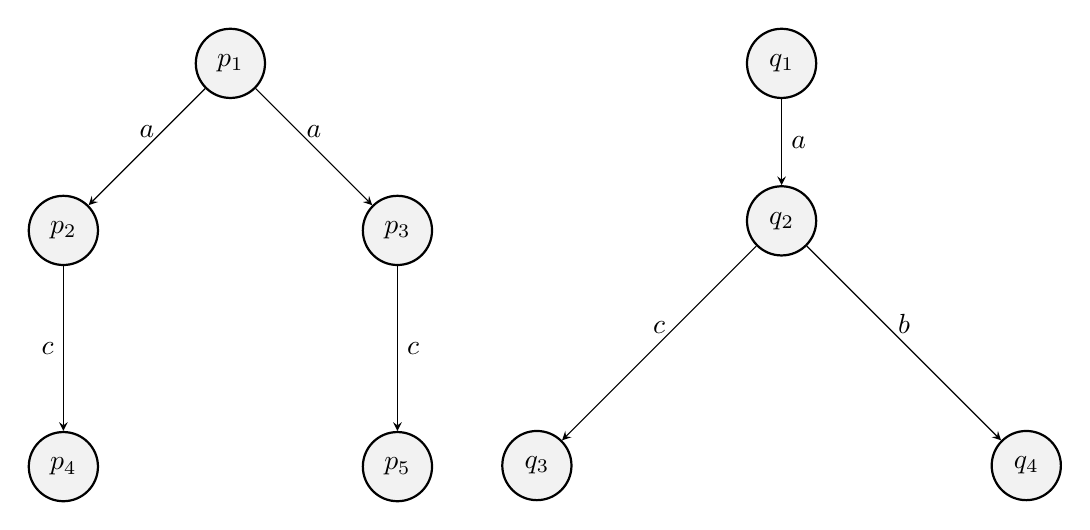
\begin{tikzpicture}
\tikzset{
->, % makes the edges directed
>=stealth, % makes the arrow heads bold
node distance=3cm, % specifies the minimum distance between two nodes. Change if necessary.
every state/.style={thick, fill=gray!10}, % sets the properties for each ’state’ node
initial text=$ $, % sets the text that appears on the start arrow
}
	\node[state] (p1) {$p_1$};
	\node[state, below left of=p1, node distance=3cm] (p2) {$p_2$};
	\node[state, below right of=p1, node distance=3cm] (p3) {$p_3$};
	\node[state, below of=p2, node distance=3cm] (p4) {$p_4$};
	\node[state, below of=p3, node distance=3cm] (p5) {$p_5$};
	\node[state, right of=p1, node distance=7cm] (q1) {$q_1$};
	\node[state, below of=q1, node distance=2cm] (q2) {$q_2$};
	\node[state, below left of=q2, node distance=4.395cm] (q3) {$q_3$};
	\node[state, below right of=q2, node distance=4.395cm] (q4) {$q_4$};
	
	\draw (p1) edge[above] node{$a$} (p2)
	(p1) edge[above] node{$a$} (p3)
	(p2) edge[left] node{$c$} (p4)
	(p3) edge[right] node{$c$} (p5)
	(q1) edge[right] node{$a$} (q2)
	(q2) edge[above] node{$c$} (q3)
	(q2) edge[above] node{$b$} (q4);
\end{tikzpicture}
\end{center}
这里不满足$(p_3, q_2) \notin R$.
\end{example}


\begin{definition}
\rm (\redt{Bisimilarity}) Given two states $p$ and $q$ in $S$, $p$ is bisimilar to $q$, written $p \sim q$,  if and only if there is a bisimulation $R$ such that $(p,q) \in R$. 
\end{definition}

\begin{definition}
\rm The bisimilarity relation $\sim$ is the union of all bisimulations.
\end{definition}

\begin{lemma}
\rm The bisimulation has some properties:
\begin{itemize}
	\item The identity relation $\vn{id}$ is a bisimulation(with two same LTS).
	\item The empty relation $\perp$ is a bisimulation.
	%\item The relation composition $R_1 \circ R_2$ of two bisimulation $R_1$ and $R_2$ is a bisimulation.
	\item (\redt{closed under union}) The $\bigcup_{i \in I} R_i$ of a family of bisimulations $(R_i)_{i \in I}$ is a bisimulation.
\end{itemize}
\end{lemma}

\begin{lemma}
\rm \cite{AITBAC} The bisimilarity relation $\sim$ is equivalence relation (i.e., reflexivity, symmetry, transitivity).
\end{lemma}

\begin{proof}
\rm 其中reflexivity, symmetry是比较显然的. Transitivity稍微麻烦一点,我们用relation composition定义新的relation$R_3 = R_1;R_2$, 此时有$(p,q) \in R_3$,因此只要证明$R_3$ is bisimulation足够了. 取任意一个$(p_1, q_1) \in R_3$,那么按照$R_3$的定义, 存在$(p_1, r_1) \in R_1$和$(r_1, q_1)$. 由$p_1 \sim r_1$那么对于任意的$p_1 \xrightarrow{\alpha} p_1'$, 存在$r_1 \xrightarrow{\alpha} r_1'$满足$(p_1',r_1') \in R_1$. 再由$r_1 \sim q_1$, 存在$q_1 \xrightarrow{\alpha} q_1'$满足$(r_1',q_1') \in R_2$. 于是按照$R_3$的定义也有$(p_1', q_1') \in R_3$. 再由$R_2$ is bisimulation, 从$(r_1,q_1) \in R_2$按照上述的思路往回证明即可,最终$R_3$ is bisimulation.
\end{proof}

\begin{definition}
\rm \cite{mLTS} An LTS is called \redt{deterministic} if for every state $p$ and action $\alpha$, there is at most one state $q$ such that $p \xrightarrow{\alpha} q$.
\end{definition}

\begin{lemma}
\rm In a deterministic LTS, two states are bisimilar if and only if they are trace equivalent,
\[
	s_1 \sim s_2 \iff \vn{Tr}(s_1)=\vn{Tr}(s_2)
\]
\end{lemma}

\begin{proof}
\rm 

先证$\Rightarrow$, 设满足$s_1 \sim s_2$($(s_1,s_2) \in R$ and $R$ is bisimultaion), 设$\sigma_{s_1} \in \vn{Tr}(s_1)$, 其中$\sigma_{s_1}$为sequence $(\alpha_i)_{i \in I}$ where $I$ is a indexed famliy. 由于$s_1 \sim s_2$, 那么对于$s_1 \xrightarrow{\alpha_1} s_1'$, 存在$s_2 \xrightarrow{\alpha_1} s_2'$, 于是$(s_1',s_2') \in R$, 根据$\sigma$长度做induction可以证明$\sigma_{s_1} \in \vn{Tr}(q)$. 再反过来证明$\sigma_{s_2} \in \vn{Tr}(s_2)$也同样有$\sigma_{s_2} \in \vn{Tr}(s_1)$. 最终$\vn{Tr}(s_1)=\vn{Tr}(s_2)$.

对于$\Leftarrow$, 我们可以用$\vn{Tr}(s_1) = \vn{Tr}(s_2)$构造一个bisimulation, 定义relation $R$为
\[
 	\vn{Tr}(s_1) = \vn{Tr}(s_2) \iff (s_1,s_2) \in R.
\]
只要能证明$R$ bisimulation即可. 首先我们来说明在deterministic限制下一个比较好性质: 若$\vn{Tr}(s_1) = \vn{Tr}(s_2)$且当$s_1 \xrightarrow{\alpha} s_1', s_2 \xrightarrow{\alpha} s_2'$, 那么$\vn{Tr}(s_1') = \vn{Tr}(s_2')$. 这样对于任意地$(s_1,s_2) \in R$, 它们accept相同action对应的transition $(s_1', s_2') \in R$. 因此$s_1 \sim s_2$. 
\end{proof}


\begin{definition}
\rm (\redt{Weak Bisimultation}) Given two labelled transition system $(S_1, \Lambda, \to_1)$ and $(S_2, \Lambda, \to_2)$, relation $R \subseteq S_1 \times S_2$ is a bisimulation iff both $R$ and its converse $\overline{R}$ are simulations, for all $(p,q) \in R$ and $\alpha \in \Lambda \cup \{\tau\}$ satisfies
\[
	\begin{gathered}
	\text{for any}~p \xrightarrow{\alpha}_1 p', ~\text{then there exists}~ q'~\text{such that}~q \xrightarrow{\tau*~\alpha~\tau*}_2^* q'~\text{and}~(p',q') \in R \\
	\text{for any}~q \xrightarrow{\alpha}_2 q', ~\text{then there exists}~ p'~\text{such that}~p \xrightarrow{\tau*~\alpha~\tau*}_1^* p'~\text{and}~(p',q') \in R
	\end{gathered} 	
\]
where $\xrightarrow{}^*$ is multi-transition.
\end{definition}


\begin{annotation}
\rm \bluet{对于LTS的一些想法}:
\begin{itemize}
	\item 如果你想用transition system来做reasoning可以考虑把它和Kripke frame联系起来,同时要构造一些modality来设计方便做reasoning的calculus.
	\item (\emph{bisimulation proof method}) 对于两个特别的states来说,我们应该如何找到这样bisimulation来满足$(p,q) \in R$?
	\item 对于两个特别的LTS来说,我们怎样以bisimulation思考它们是否equivalent? bisimulation的最初定义应该叫做strong bisimulation, 它建立的是一种strong equivalence, 而weak bisimulation建立是一种observation equivalence.
\end{itemize}
\end{annotation}

\begin{annotation}
\rm  \todo{CCS(calculus of communicating systems)\cite{CCS} and mCRL2 \cite{mLTS}}.
\end{annotation}

\newpage
\section{Symbolic Execution}

\subsection{Predicate transformer}

\begin{definition}
\rm A \redt{predicate transformer} $p$ is a function
\[
    p: \text{FOL} \times \text{stmts} \to \text{FOL}
\]
where FOL are first-order logic formulas and stmts are program statements.
\end{definition}

\begin{definition}
\rm Given a FOL $Q$ and program statement $c$, the \redt{weakest precondition} is a FOL $\text{wp}(Q, c)$ satisfies the following conditions
\begin{itemize}
    \item $\{\text{wp}(Q, c)\}c\{Q\}$.
    \item for any FOL $P$ such that $\{P\}c\{Q\}$, $P \Rightarrow \text{wp}(Q, c)$.
\end{itemize}  
\end{definition}

\begin{example}
\rm For assumption 
\[
    \text{wp}(Q, \text{assume}~e\} = e \to Q,
\]
想想deduction theorem或者modus ponens, 没有比这个更弱的.  
\end{example}

\begin{definition}
\rm Given a FOL $Q$ and program statement $c$, the \redt{strongest postcondition} is a FOL $\text{sp}(P, c)$ satisfies the following conditions
\begin{itemize}
    \item $\{P\}c\{\text{sp}(Q, c)\}$.
    \item for any FOL $Q$ such that $\{P\}c\{Q\}$, $\{\text{sp}(Q, c)\} \Rightarrow Q$.
\end{itemize}
\end{definition}

\begin{example}
\rm For assignment, there is standard nation. One possible is  
\[
    \text{sp}(P[e/x], x \coloneqq e) = P.
\]
Another one is 
\[
    \text{sp}(P, x \coloneqq e) \equiv \exists v'. v = e[v'/v] \wedge P[v'/v].
\]
For example, 
\[
    \text{sp}(x \geq i, x \coloneqq x+k) \equiv (\exists x'. x = x' + k \wedge x' \geq i) \equiv (x-k \geq i). 
\]
第二种方式显的更加的自然, 对做符号执行是比较友好的.  
\end{example}



\subsection{Some Reasoning}

\begin{example}
\rm \redt{Symbolic reachability analysis} 这是来自\cite{BMGM15}的一个小例子, 我们尝试用dynamic symbolic execution做一些reasoning. 
\begin{minted}[tabsize=4,linenos, frame=single, fontsize=\small]{c}
#define VALVE_KO(status) status == -1 
#define TOLERANCE 2  
extern int size; 
extern int valvesStatus[];  

int getStatusOfValve(int i){ 
	if(i < 0 || i >= size){ 
		printf ("ERROR"); 
		exit(EXIT_FAILURE); 
	}
	int status = valvesStatus[i]; 
	return status; 
} 

int checkValves(int wait1, int wait2) { 
	int count, i; 
	while(wait1 > 0) wait1--; 
	count = 0, i = 0; 
	while(i < size){ 
		int status = getStatusOfValve(i);
	
		if(VALVE_KO(status)) {
			count++;
		}
		i++;
	}
	
	if(count > TOLERANCE)
		printf ("ALARM");
	}
	while(wait2 > 0) wait2--; 
		return count;
\end{minted}
\cite{BMGM15}提到了一个symbolic reachability analysis, 它和我们常见的symbolic execution是不一样的, 它可以看做给定一个postcondition沿着control flow往后推. 这种方法在解决一些branch condition indirectly related to input, 可能会有一些帮助. 例如L29所在branch condition, 它并不是直接依赖input. 如果我们将这个while展开,那么每次在某条路径上做symoblic execution到L28时, count都是一个concrete value, 如果想尝试在L28这里开分支是做不到的.    

例如我们想进入L29所在的branch, 那么one-step induction如下:
\begin{minted}[mathescape=true, tabsize=4, frame=single, fontsize=\small]{c}
// $P_{28} = count > 2$
{L28: count > 2}
// $Q_{28} = true$
\end{minted}
可以看到precondition是weakest的, 后面推导依然保持这个性质. 继续往后推导我们需要尝试得resolve掉L19-L26的while, 这里可能就有infinitely many paths, 例如执行$0,1,2,\cdots$次这个loop. 顺着这个思路来选择路径往后做symbolic execution, 路径直到function entry为结束.
\begin{minted}[mathescape=true, tabsize=4, frame=single, fontsize=\small]{c}
//Path_1: L15-> L16 -> L17 -> L18 -> L19 -> L28

// $P_{18} = count > 2 \wedge i \geq size \wedge 0 > 2 \wedge 0 > size \equiv false$
{L18: count = 0, i = 0; }
// $Q_{18} = count > 2 \wedge i \geq size$
// $P_{19} = count > 2 \wedge i \geq size$
{L19: i >= size}
// $Q_{19} = count > 2$ 
// $P_{28} = count > 2$
{L28: count > 2}
// $Q_{28} = true$
\end{minted}
在$P_{18}$这里得到了一个contradiction, 这就意味着上面选择的path是infeasible的,那么到这里我们就不能往后再继续推理了. 现在我们给用$Ln_{a}, Ln_{b},\cdots$的形式来表示对同一statement $Ln$ 的多次执行.
\begin{minted}[mathescape=true, tabsize=4, frame=single, fontsize=\small]{c}
//Path_2: $\cdots$ -> L$19_b$ -> L$20_b$ -> L$22_b$ -> L$23_b$ -> L$25_b$ -> L$19_a$ -> L28

...
// $P_{19b} = count > 1 \wedge i = size-1 \wedge i \geq 0 \wedge valvesStatus[i] = -1 \wedge i < size$
{L19b: i < size}
// $Q_{20b} = count > 1 \wedge i = size-1 \wedge i \geq 0 \wedge valvesStatus[i] = -1$
// $P_{20b} = (count > 1 \wedge i \geq size -1 \wedge i \geq 0 \wedge i < size \wedge valvesStatus[i] = -1) \equiv$
// $(count > 1 \wedge i = size-1 \wedge i \geq 0 \wedge valvesStatus[i] = -1)$
{L20b: int status = getStatusOfValve(i);}
// $Q_{20b} = count > 1 \wedge i \geq size -1 \wedge status = -1$
// $P_{22b} = count > 1 \wedge i \geq size -1 \wedge status = -1$
{L22b: status == -1}
// $Q_{22b} = count > 1 \wedge i \geq size -1$
// $P_{23b} = (count+1 > 2 \wedge i \geq size -1) \equiv (count > 1 \wedge i \geq size -1)$
{L23b: count++}
// $Q_{23b} = count > 2 \wedge i \geq size-1$
// $P_{25b} = (count > 2 \wedge i+1 \geq size) \equiv (count > 2 \wedge i \geq size-1)$ 
{L25b: i++; }
// $Q_{25b} = count > 2 \wedge i \geq size$
// $P_{19a} = count > 2 \wedge i \geq size$
{L19a: i >= size}
// $Q_{19a} = count > 2$ 
// $P_{28} = count > 2$
{L28: count > 2}
// $Q_{28} = true$
\end{minted}
上面就是执行了最后一次循环并且在这次循环中进入了L23所在的branch,主要需要注意一下$P_{20b}$这里设计到了inter-analysis. 
\end{example}


\newpage
\subsection{Craig Interpolation}

\begin{definition}
\rm Let $P \to Q$ be a valid propositional formula. A Craig Interpolation for $P$ and $Q$ is a formula $C$ that satisfies the following conditions:
\begin{itemize}
	\item $P \to C$ and $C \to Q$ are valid.
	\item All the variables in $C$ also appear in both $P$ and $Q$.
\end{itemize}
\end{definition}

\begin{theorem}
\rm (\redt{Craig Interpolation Theorem}) Let $P \to Q$ be a propositional formula, where $P$ and $Q$ share at least one atomic proposition. Then there exists a formula $C$ containing only variable symbols in both $P$ and $Q$ such that $P \to C$ and $C \to Q$.
\end{theorem}

\begin{proof}
\rm 我们用$\text{atoms}(P)$和$\text{atoms}(Q)$分别表示$P$和$Q$中的variable symbols(atomic proposition). 这里对$|\text{atoms}(P)-\text{atoms}(Q)|$做induction, 其中$\text{atoms}(P)-\text{atoms}(Q)$表示出现在$P$中但不在$Q$中的variable symbols.  

\textsc{Base case}: 当$|\text{atoms}(P)-\text{atoms}(Q)| = 0$, 我们可以让$C = P$作为一个interpolation,显然$P \to P$ is valid and $P \to Q$.

\textsc{Inductive hypothesis}: 假设$|\text{atoms}(P)-\text{atoms}(Q)| = n$时原命题成立.

\textsc{Inductive case}: 当$|\text{atoms}(P)-\text{atoms}(Q)| = n+1$时,我们取$\alpha \in |\text{atoms}(P)-\text{atoms}(Q)|$.  我们定义$P_{\alpha \mapsto \top}$表示将$P$中所有$\alpha$替换成$\top$得到的formula, 类似地我们用$P_{\alpha \mapsto \bot}$表示将$P$中所有$\alpha$替换成$\bot$得到的formula. 显然我们有$P \equiv P_{\alpha \mapsto \top} \vee P_{\alpha \mapsto \bot}$. 根据inductive hypothesis我们找到一个关于$P_{\alpha \mapsto \top} \vee P_{\alpha \mapsto \bot} \to Q$的interpolation $C$. 显然$C$也是$P \to Q$的一个interpolation.
\end{proof}

\begin{annotation}
\rm 值得注意上面的proof仅仅在proposition logic下证明了Craig interpolation了. 这也是为什么我们可以将上面的$\alpha$分别用$\top$和$\bot$替换,因为$\alpha$表示的实际是atomic proposition, 对于atomic proposition而言它只有$\top$和$\bot$.

那么比较自然的问题就是first-order logic上怎么证明? 先回答两个first-order formula $\varphi$和$\psi$需要shared什么? 若
\[
\forall x. F(x)  \to \exists y. F(y). 
\]
\cite{CF2007}里面提到了non-logical symbols, 那么first-order logic中的non-logical symbols到底是什么呢? 在wiki中它被定义为predicates, functions, and constants. 我们来分别思考一下这些symbols在上面的inductive step中应该怎么被处理? 
\begin{enumerate}
	\item 如果存在constant $c_1 \in \text{atoms}(P)-\text{atoms}(Q)$, 此时我们可以用新一个fresh variabe $v_1$来替换这个$c_1$, 得到一个新的formula $\exists v_1. P_{c_1 \mapsto v_1}$. 显然$P \to \exists v_1. P_{c_1 \to v_1}$, 这里就可以继续用inductive hypothesis了.
	\item 如果存在function $f_1 \in \text{atoms}(P)-\text{atoms}(Q)$, ???
	\item 如果存在predicate $p_1 \in \text{atoms}(P)-\text{atoms}(Q)$, ???
\end{enumerate}
看来并不trivial. 这里需要再想想.
\end{annotation}

\begin{theorem}
\rm (\redt{Satisfiability form}) Let $A$ and $B$ be proposition formula. A Craig Interpolation for $A$ and $B$ is a formula that satisfies the follow:
\begin{itemize}
	\item $A \wedge B$ is unsatifiable.
	\item $A \to C$.
	\item $C \wedge B$ is unsatifiable.
\end{itemize}
\end{theorem}

\begin{annotation}
\rm 如何理解上面的satisfiability form呢? 首先$A \wedge B$ is unsat, 那么则有$(\neg A \vee \neg B) \equiv (A \to \neg B)$ is valid. 再$C \vee B$ is unsat, 那么则有$(\neg C \vee \neg B) \equiv (C \to \neg B)$ is valid. 显然$C$是关于$A$和$\neg B$的一个interpolation.

在使用中我们会通常中$A$和$B$分别表示两个set of clauses, 也就是对$A$和$B$进行normalization先.  
\end{annotation}

\begin{definition}
\rm A proof of unsatisifability $\varPi$ for a set of clause $C$ is a root-tree $(V_\varPi, E_\varPi)$, where $V_\varPi$ is a set of clauses, such that for every vertex $c \in V_{\varPi}$:
\begin{itemize}
	\item if $c$ is a empty clause, then $c$ is the unique root.
	\item if $c$ is resolvent of $c_1$ and $c_2$, then edge $(c,c_1)$ and $(c,c_2)$ are both in $E_\varPi$.
	\item $c$ is leaf that is caluse in $C$ otherwise.
\end{itemize}
\end{definition}

\begin{annotation}
\rm 这个proof实际就是做resolution得到empty clause一个过程, 是很自然的一个从下到上的一棵树, 当然也有定义把empty clasue当做unique leaf的形式. 无论哪种情况,只要能理解resolution过程就行. 这里简单把resolution再写一遍.
\[
	\infer{C_1 \cup C_2}{p \cup C_1 & \neg p \cup C_2}
\]
其中literal $p$对应的variable称为pivot variable.
\end{annotation}

\begin{definition}
\rm Given a set of clauses $C$, we say a variable is \redt{global} if it appears in all clauses in $C$, and \redt{local} to one clause $c$ in $C$ if it appear only in $c$. Given any clause $c_i \in C$, we denote by $g(c_i)$ the disjunction of the \redt{global literals} in $c_i$ and by $l(c_i)$ the disjunction of \redt{literals local} to $c_i$ 
\end{definition}

\begin{annotation}
\rm 注意上面variable和literal的描述. 
\end{annotation}

\begin{theorem}
\rm (\redt{linear-time construction}) Let $(A,B)$ be a pair of caluse sets and let $\varPi$ be a proof of unsatisfiability of $A \cup B$. For all vertices $c \in V_{\varPi}$, let $p(c)$ be a boolean formula, such that 
\begin{itemize}
	\item if $c$ is leaf, then
	\begin{itemize}
		\item if $c \in A$ then $p(c) = g(c)$,
		\item else $p(c)$ is the $\top$.
	\end{itemize}
	\item else, let $c$ is resolvent of $c_1$ and $c_2$ and let $v$ be pivot variable of this resolution. 
	\begin{itemize}
		\item if $v$ is local to $A$, then $p(c) = p(c_1) \vee p(c_2)$,
		\item else $p(c) = p(c_1) \wedge p(c_2)$.
	\end{itemize}
\end{itemize}
Then $p(\bot)$ is an interpolant for $(A, B)$ where $\bot$ is the root of $\varPi$.
\end{theorem}


\makeatletter
\DeclareRobustCommand{\lvdots}{%
  \vbox{
    \baselineskip6\p@\lineskiplimit\z@
    \kern-\p@
    \hbox{.}\hbox{.}\hbox{.}\hbox{.}\hbox{.}\hbox{.}\hbox{.}\hbox{.}\hbox{.}
  }}
\makeatother

\begin{annotation}
\rm 这个证明感觉不是那么显然, 花了2-3天想了一下. 先从直觉出发,我们先设$A$和$B$是没有common clauses,再假设proof $\varPi$里面属于$A$的leaves为$\{\alpha_1, \alpha_2, \cdots, \alpha_m\}$, 属于$B$的leaves为$\{\beta_1, \beta_2, \cdots, \beta_n\}$. 我们可以重排整个proof $\varPi$: 
\begin{itemize}
	\item 先对$\{\alpha_1, \alpha_2, \cdots, \alpha_m\}$做resolution, 直到无法继续. 得到$\{\alpha_1', \alpha_2', \cdots, \alpha_i'\}$
	\item 再对$\{\alpha_1', \alpha_2', \cdots, \alpha_i'\}$和$\{\beta_1, \beta_2, \cdots, \beta_n\}$一起做resolution.
\end{itemize}
上述想法实际对应了这样一个操作,如果$\varPi$中存在这样一个片段:
\[
	\infer[v_1 \in l(A)]{c_1}{\infer[v_1 \notin l(A)]{v_1 \cup c_2}{\deduce{v_2 \cup c_4}{\mathcal{D}} & \deduce{\neg v_2 \cup c_5}{\mathcal{E}}} & \deduce{\neg v_1 \cup c_3}{\mathcal{F}}}
\]
我们就把下面这个resolution往上移动,变成下面这样
\[
	\begin{aligned}
	\infer[v_2 \notin l(A)]{c_1}{\infer[v_1 \in l(A)]{v_2 \cup (c_4 \backslash v_1 \cup c_3)}{\deduce{v_1 \cup (v_2 \cup c_4 \backslash v_1)}{\mathcal{D}} & \deduce{\neg v_1 \cup c_3}{\mathcal{F}}} & \deduce{\neg v_2 \cup c_5}{\mathcal{E}}}\\ 
	\infer[v_2 \notin l(A)]{c_1}{\deduce{v_2 \cup c_4 }{\mathcal{D}} & \infer[v_1 \in l(A)]{\neg v_2 \cup (c_5 \backslash v_1 \cup c_3)}{\deduce{v_1 \cup (\neg v_2 \cup c_5 \backslash v_1)}{\mathcal{E}} & \deduce{\neg v_1 \cup c_3}{\mathcal{F}}}}
	\end{aligned}
\]
上面两个略微不同的形式依赖于$c_1$到底是在$c_4$里面还是在$c_5$里面. 显然这个往上移动操作是可以做到的,也就是说现在整棵树依然是$(A,B)$一个proof, 我们设其为$\varPi'$, 我们接着来研究一下两个proof最后得到的$p(\bot)$有什么关系, 我们设$\varPi'$对应$p'(\bot)$. 因为上述只是一个局部变换,没有新增任何结点,只有两个结点对应的boolean formula发生了变化,对于整个proof而言只是以$c_1$为根结点的子树发生了变化,所以我们只需要看一下$p(c_1)$和$p'(c_1)$到底是什么关系. 我们先设$p(v_2 \cup c_4) = b_1, p(\neg v_2 \cup c_5) = b_2, p(\neg v_1 \cup c_3) = b_3$. 那么显然$p(c_1) = (b_1 \wedge b_2) \vee b_3$. 对于$p'(c_1)$我们有两个不同的结果:
\begin{itemize}
	\item $v_1 \in c_4$: $p_1'(c_1) = b_1 \wedge (b_3 \vee b_2) \equiv (b_1 \wedge b_3) \vee (b_1 \wedge b_2)$
	\item $v_2 \in c_5$: $p_2'(c_2) = (b_1 \vee b_3) \wedge b_2 = (b_1 \wedge b_2) \vee (b_2 \wedge b_3)$
\end{itemize}
显然有$p_1'(c_1) \to p(c_1)$和$p_2'(c_1) \to p(c_1)$. 这可以说明什么呢? $p'(\bot) \to p(\bot)$, 很可惜这种方式只能得到上述定理的一个弱的形式. 换句话就是我们只能得到一个比较强的interpolation,我们一般更在乎是尽量弱的interpolation, 这样它的结构或许更加的简洁.


换个思路我们重新开始思考,既然上面那个方向转换不行,我们换个方向. 我们这样重排 proof $\prod$:
\begin{itemize}
	\item 先对$\{\beta_1, \beta_2, \cdots, \beta_n\}$做resolution,直到无法继续. 得到$\{\beta_1', \beta_2', \cdots,\beta_j'\}$.
	\item 再对$\{\beta_1', \beta_2', \cdots,\beta_j'\}$和$\{\alpha_1, \alpha_2, \cdots, \alpha_m\}$一起做resolution.
\end{itemize}
但是这里有一个小问题就是pivot variable为$v_1 \notin l(A)$的resolutions并不完全是$B$里面的resolution,当$v_1$是global variables的时候它实际是属于$A$与$B$之间的resolution. 这里其实就暗示了我们需要对上面的第二步再细化一步, 这个问题留到后面. 我们先看看反方向移动有什么性质. 如果$\varPi$中存在这样一个片段:
\[
	\infer[v_1 \notin l(A)]{c_1}{\infer[v_1 \in l(A)]{v_1 \cup c_2}{\deduce{v_2 \cup c_4}{\mathcal{D}} & \deduce{\neg v_2 \cup c_5}{\mathcal{E}}} & \deduce{\neg v_1 \cup c_3}{\mathcal{F}}}
\]
我们把下面resolution还是往上移动,变成下面这样:
\[
	\begin{aligned}
	\infer[v_2 \in l(A)]{c_1}{\infer[v_1 \notin l(A)]{v_2 \cup (c_4 \backslash v_1 \cup c_3)}{\deduce{v_1 \cup (v_2 \cup c_4 \backslash v_1)}{\mathcal{D}} & \deduce{\neg v_1 \cup c_3}{\mathcal{F}}} & \deduce{\neg v_2 \cup c_5}{\mathcal{E}}}\\ 
	\infer[v_2 \in l(A)]{c_1}{\deduce{v_2 \cup c_4 }{\mathcal{D}} & \infer[v_1 \notin l(A)]{\neg v_2 \cup (c_5 \backslash v_1 \cup c_3)}{\deduce{v_1 \cup (\neg v_2 \cup c_5 \backslash v_1)}{\mathcal{E}} & \deduce{\neg v_1 \cup c_3}{\mathcal{F}}}}
	\end{aligned}
\]
实际就是把前面的$\notin$和$\in$互换. 此时有$p(c_1) = (b_1 \vee b_2) \wedge b_3$. 对于$p'(c_1)$分别有
\begin{itemize}
	\item $c_1 \in c_4$: $p_1'(c_1) = (b_1 \wedge b_3) \vee b_2 $.
	\item $c_1 \in c_5$: $p_2'(c_2) = b_1 \vee (b_3 \vee b_2)$.
\end{itemize}
显然此时我们有了希望看到的结论$p(c_1) \to p'(c_1)$, 等价于我们已经有了$p(\bot) \to p'(\bot)$这已经算是成功的基础了). 当你不断对proof $\varPi$做这个操作,直到无法继续我们设这个新的proof为$\varPi'$. 现在我们来看一下$\varPi'$结构是怎样的. 现在$\varPi$最上面的resolution都是pivot variable都满足$v \notin l(A)$,前面也提到了这样的resolution包含了pivot variable $v \in l(B)$和$v \in g(A)$两种情况. 我们再来排一次,把pivot variable $v \in l(B)$放在最前面. 也就是如出现下述proof片段:
\[
	\infer[v_1 \in l(B)]{c_1}{\infer[v_1 \in g(A)]{v_1 \cup c_2}{\deduce{v_2 \cup c_4}{\mathcal{D}} & \deduce{\neg v_2 \cup c_5}{\mathcal{E}}} & \deduce{\neg v_1 \cup c_3}{\mathcal{F}}}
\]
我们把下面resolution往上移动, 也会得到上述类似两种形式, 这里不在累述了. 最重要是此时$p'(c_1) = p''(c_1)$, 因为这里都是conjunction. 这就是说明这种移动并不会影响对应结点的boolean formula, 也就是说依然有$p(c_1)\to p''(c_1)$. 我们对$\varPi'$不断做这个操作,知道无法继续我们设这个新的proof为$\varPi''$. 我们可以简单画一下$\varPi''$的结构:
\[
	\deduce[\lvdots^{v \in l(A)}]{\bot}{\deduce[\lvdots^{v \in g(A)}]{\gamma_1 \quad \cdots \quad \gamma_s}{\deduce[\lvdots^{v \in l(B)}]{\beta_1' \quad \cdots \quad \beta_j'}{\beta_1 & \cdots & \beta_m} & \alpha_{i_1} & \cdots & \alpha_{i_k}} & \alpha_{t_1} & \cdots & \alpha_{t_l}}
\]
整个结构分为三个层次,是我们通过前两次移动策略得到的. 我们主要看一下中间整个层次. 首先可以确定是$\{\beta_1',\cdots, \beta_j'\}$里面所有variables都是在$g(A)$中, 此时我们如果考虑把$\alpha_{i_1}, \cdots , \alpha_{i_k}$分布替换成$g(\alpha_{i_1}), \cdots,  g(\alpha_{i_k})$. 此时第二个层次的结构是不会发生变化的,因为它里面做的resolution的pvoit variables也都在$g(A)$. 并且你会发现${\gamma_1, \cdots, \gamma_s}$会被消成$\bot$. 这样我们得到又得到了一个新的更短的proof $\varPi'''$,我们也自然地得到了一个interpolation $g(\alpha_{i_1}) \wedge \cdots \wedge g(\alpha_{i_k})$. 我们证明了一个比较弱的interpolation,那么原来比它强的interpolation也自然是存在的,这样我们整个证明就结束了.
\end{annotation}

\begin{proof}
\rm Formalization for above sketch.
\end{proof}

\begin{annotation}
\rm 上面的theorem最重要地就是告诉我们计算interpolation不需要第二次用到SAT-solver, 并且整个计算过程是线性的. 
\end{annotation}

\begin{definition}
\rm (\redt{Craig interpolant over path}) Given formula $A_1 \wedge A_2 \wedge \cdots \wedge A_n$ is unsatisfiable. Let sequence of formulas $\hat{A}_0, \hat{A}_1, \cdots, \hat{A}_n$ is defined as follows.
\begin{itemize}
	\item $\hat{A}_0 = true$ and $\hat{A}_n = false$. 
	\item for all $1 \leq i \leq n$, $\hat{A}_{i-1} \wedge A_i \to \hat{A}_{i}$.
	\item for all $1 \leq i < n$, $\hat{A}_i \in (\mathcal{L}(A_1 \wedge \cdots \wedge A_i) \cup \mathcal{L}(A_{i+1} \wedge \cdots \wedge A_n))$ where $\mathcal{L}(\phi)$ denote well-formed formula over the vocabulary of $\phi$.
\end{itemize}
\end{definition}

%\begin{annotation}
%\rm 路径条件通常形如canonical form $A_1 \wedge A_2 \wedge \cdots \wedge A_n$. 当通过SAT-slover对其求解得到结果是unsatisfiable, 意味这这样的路径是unreachable的. 于是我们可以把这样的路径排除在后续的分析之外, 排除在外的手法有很多.
%\end{annotation}

\newpage
\subsection{Graph as Proof}

\begin{annotation}
\rm 当我们想证明program中某个点unreachable的时候,我们需要说明可以抵达这个点的所有路径都是infeasible的. 那么我们应当以怎样的形式给出这个证明呢? 我们可以从CFG构造出另外一个graph, 借助这个graph我们可以很直接说明这些路径确实不存在, 这里有两种手法:
\begin{itemize}
	\item 直接在graph上显式地去掉这些路径.
	\item graph上显式的把这些路径标出来,并且说明这些路径不存在.
\end{itemize}
无论哪种方法都需要扩展原CFG. 我们可以形式化一点,设CFG为$G_1 = (V_1,E_1)$和新的graph为$G_2 = (V_2, E_2)$. 我们需要两个basic map:
\begin{itemize}
	\item vertex map: $f_v: V_2 \to V_1$.
	\item edge map: $f_e: E_2 \to E_1$.
\end{itemize}
这两个map在这里指明$G_2$上vertex和edge都在$G_1$中, 因为我们希望$G_2$上的路径都是在$G_1$中的. 值得注意的是存在$f_v(v) = f(w), v \neq w \in V_2$. 这是因为希望$G_2$可以表示独立的路径,这使得我们需要把两条不同路径上的重复结点分开,这样的重复结点虽然对应$G_1$中同一个结点但是在$G_2$是distinct的.

无论哪种的方法,我们都是无法避免去选路径,然后沿着路径去分析的. 这里我们继续以符号化分析为起点,给定一条从entry noode到target node的路径$\pi = (\epsilon, a_0, a_1, \cdots, a_n)$, 它对应path condition是normal form为$P_\pi = A_0 \wedge A_1 \wedge A_n$. 我们再建立一个对应关系, 当$i > 0$时, $a_{i-1}$执行$a_i$都之前都满足需要$A_i$. 其中$a_0$是真正的entry node, 额外给出$\epsilon$为了可以在开始的时候方便地给一个initial condition(函数调用传参). 这里有两种情况:
\begin{itemize}
	\item $P_\pi$ is sat, 那么我们可以直接出给反例.
	\item $P_\pi$ is unsat, 那么我们就可以排除这条路径. 
\end{itemize}
后面我们主要研究如何不断的排除这条路径.
\end{annotation}

\begin{example}\label{ex:refine_path1}
\rm (\redt{Navie analysis}) 我们通常是在CFG类似的program graph上进行分析,显然我们分析的路径都是这个CFG上存在的路径. 当某条路径是infeasible时,我们可以想办法把它从CFG上抹去,这就是最初的直觉.
	\begin{figure}[h]
    \centering
    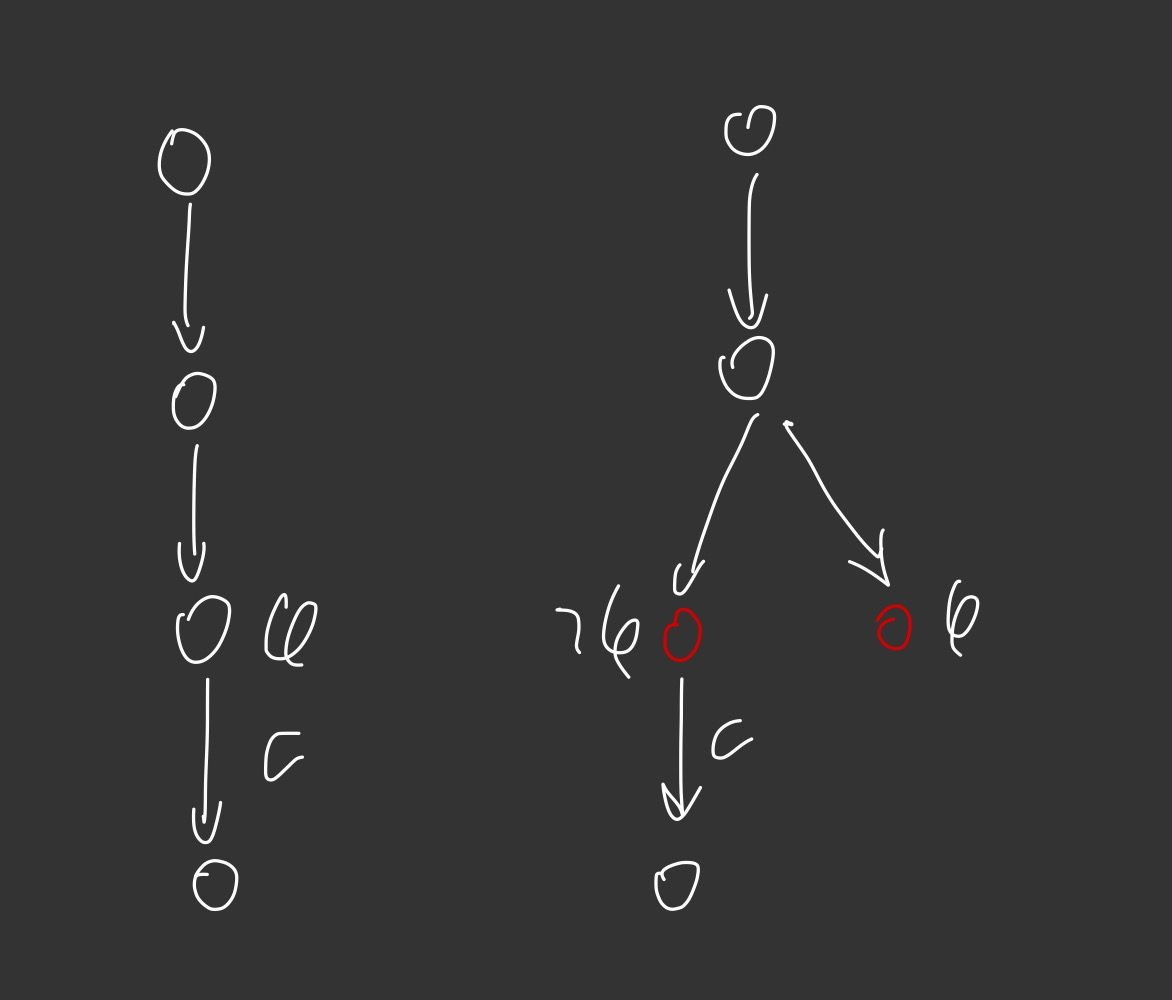
\includegraphics[width=0.4\textwidth]{images/644CA52C-1C17-4714-A076-2AE26418F4CE.jpeg}
    \caption{Refinement by node copying}
    \label{fig:refine1}
    \end{figure}
    图\ref{fig:refine1}中的$\varphi$为图中路径的prefix path condition, 消除这条路径并不能简单的把$c$这条边去掉, 我们需要copy结点然后加上annotation, 这个annotation的含义是路径条件满足它的时候才能继续往前. 因此这里带$\varphi$的copy结点是没有以$c$为label的outgoing edge. 这样在annotation + copy的模式下我们就去掉了infeasible path. 
    
  	还有一个问题是我们应该选择copy哪一个结点, 通常我们选择那个结点是和frontier相关的,frontier是一种特殊的边. 它连接的我们已知可达的结点和还没有抵达的结点, 这里我们还不知道它是否可达. 当我们经过进一步计算之后发现它不可达, i.e., 一步扩展可达路径的路径. 此时这个不可达结点的前驱可达结点,就可以称为我们的copy对象. 可以看见这个$\varphi$是满足一定性质的,即$\varphi$ is sat and $\varphi \wedge \psi_c$ is unsat, 这是有道理的. 我们不能任意选择infeasible path中间的结点来copy, 然后删掉一些边. 你必须要保证从删掉这些边产生的路径都是infeasible才行. 
    
    最后一个值得探讨的问题, 这个$\phi$往往是比较复杂的, 把它作为annotation实际上不太方便的, 因为当你抵达这个点的时候, 你需要判断它是否满足$\phi$再做进一步打算. 利用Craig interpolation我们就可以简化这个$\phi$, 得到一个$\hat{\phi}$. 在满足$\hat{\phi}$的情况下也是不可达的,这里弱一点$\hat{\phi}$显然要比$\phi$好.
    
    上面的这种方法存在冗余的问题. 举一个完整的分析例子, 图\ref{fig:refine2}对应一个带if的简单程序, 在if的出口有一个关于error的transition,假设error这个点是unreachable的,其他的点都是reachable的. 其中绿色的路径表示我们每次分析的CFG上关于error的一条路径, 这里我们用了7步才判定图中error这个点是unreachable的. 我们分别来看一下过程:
    \begin{enumerate}
    	\item 此时$\pi$取不经过if的路径. 这里$\varphi_1$ is sat and  $\varphi_1 \wedge \varphi_e$ is unsat. 那么$e$对应的这条边就是这里的froniter, 这里我们copy $\varphi$所对应的结点. 我们设copy对象为结点$v$, copy的步骤如下:
    	\begin{itemize}
    		\item copy $v$得到$v'$, 包括$v$的所有前驱都需要也指向$v'$; $v'$只需要指向所有$v$的后继.
    		\item 去掉$v$上的froniter. 
    	\end{itemize}
		$v$上标注annotation $\varphi_1$, 而$v'$上标注annotation $\neg \varphi_1$. 于是得到了(2).
		\item 此时$\pi$取(2)中经过if的路径. 这里$\neg \varphi_1 \wedge \varphi_2 \wedge \varphi_e$ is unsat. 那么$e$对应的这条边就是这里的frontier, 这里我们copy $\neg \varphi_1 \wedge \varphi_2$对应的结点, 得到$\varphi_1 \vee \neg \varphi_2$. 这里我写错成$\neg \varphi_1 \wedge \neg \varphi_2$. 理论上这个条件也没什么问题, 所以这里貌似还要多几步才行, 最终得到应该会是一个$\neg \varphi_1 \wedge (\varphi_1 \vee \neg \varphi_2)$.
    \end{enumerate}
    \begin{figure}[H]
    \centering
    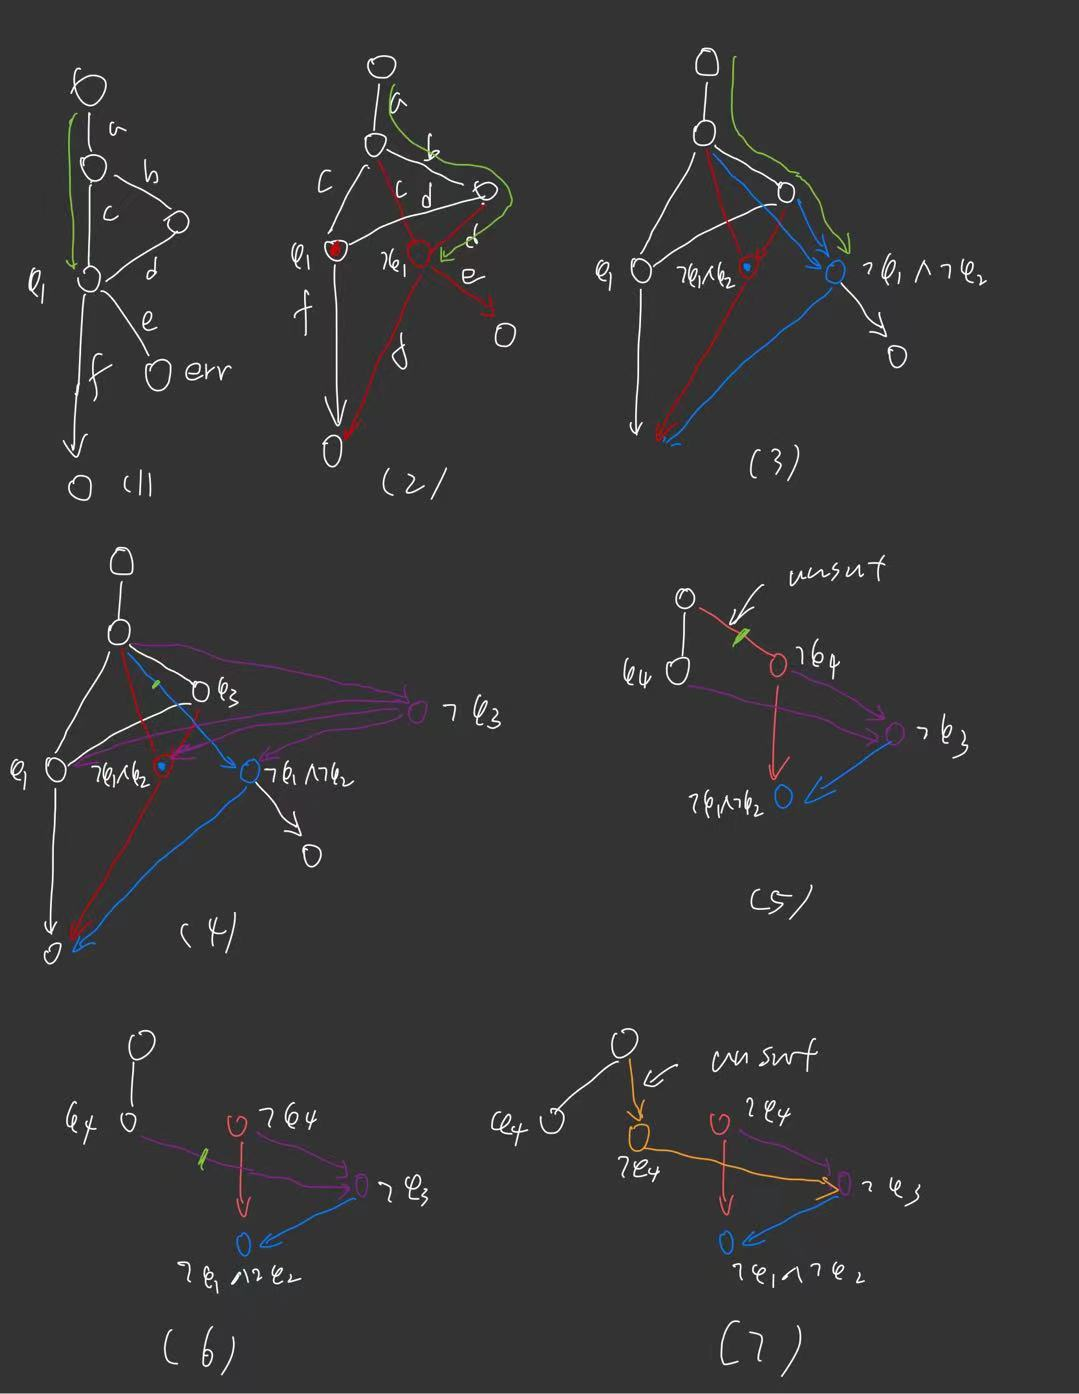
\includegraphics[width=0.8\textwidth]{images/refine2.jpeg}
    \caption{Refinement by node copying}
    \label{fig:refine2}
    \end{figure}
其余过程类似. 它显然对应了我们前面提到的第一种方法, 最后图上不存在从开始结点到error结点的显式路径. 但是分析过程是非常impractical的, 相关图的扩展几乎是成指数型的, 并且在分析过程中会发现有一些分析步骤是冗余的. 最后总结一下这种方法内在本质:
\begin{itemize}
	\item 不断地寻找frontier, 切割frontier的一段. 新增的edges可以作为新frontier,这些新增的edges包括了切割froniter一段的前驱, 这样我们实际总是在压缩前置路径. 直到frontier一端为entry node, 那么此时可选的路径就是只能是frontier本身. 如果依然是unsat, 那么就可以证明确实不存在这样的一条从entry node出发的路径.
	%\item 图\ref{fig:refine2}中的(2)图,左上角的这条红边实际是可以去掉的, 因为这样的前置路径只有一条.
	%\item 前面提到的一个问题, (1) to (2), 会将其中frontier一端的结点分割成$\varphi_1$和$\neg \varphi_1$. 接着$\neg \varphi_1$所在结点又会分割成$\neg \varphi_1 \wedge \varphi_2$和$\neg(\neg \varphi_1 \wedge \varphi_2) \equiv \varphi_1 \vee \neg \varphi_2$. 问题来了, 这里又把$\varphi_1$带回来了, 并且你要知道(2)中那条左上红色的边一直存在的. 最终这里因为这条边的存在,会继续分为$\varphi_1 \wedge (\varphi_1 \vee \neg \varphi_2) \equiv true$和$\neg (\varphi_1 \wedge (\varphi_1 \vee \neg \varphi_2)) \equiv false$. 如果我们在(2)把左上角红边作为下一步的frontier, 似乎就可以避免上述情况.
	\item 实际处理的路径要比真实存在的路径要多的. 我们想一个极端情况图\ref{fig:refine3}, 假设原CFG上只有一条指向target的路径.
	\begin{figure}[H]
    \centering
    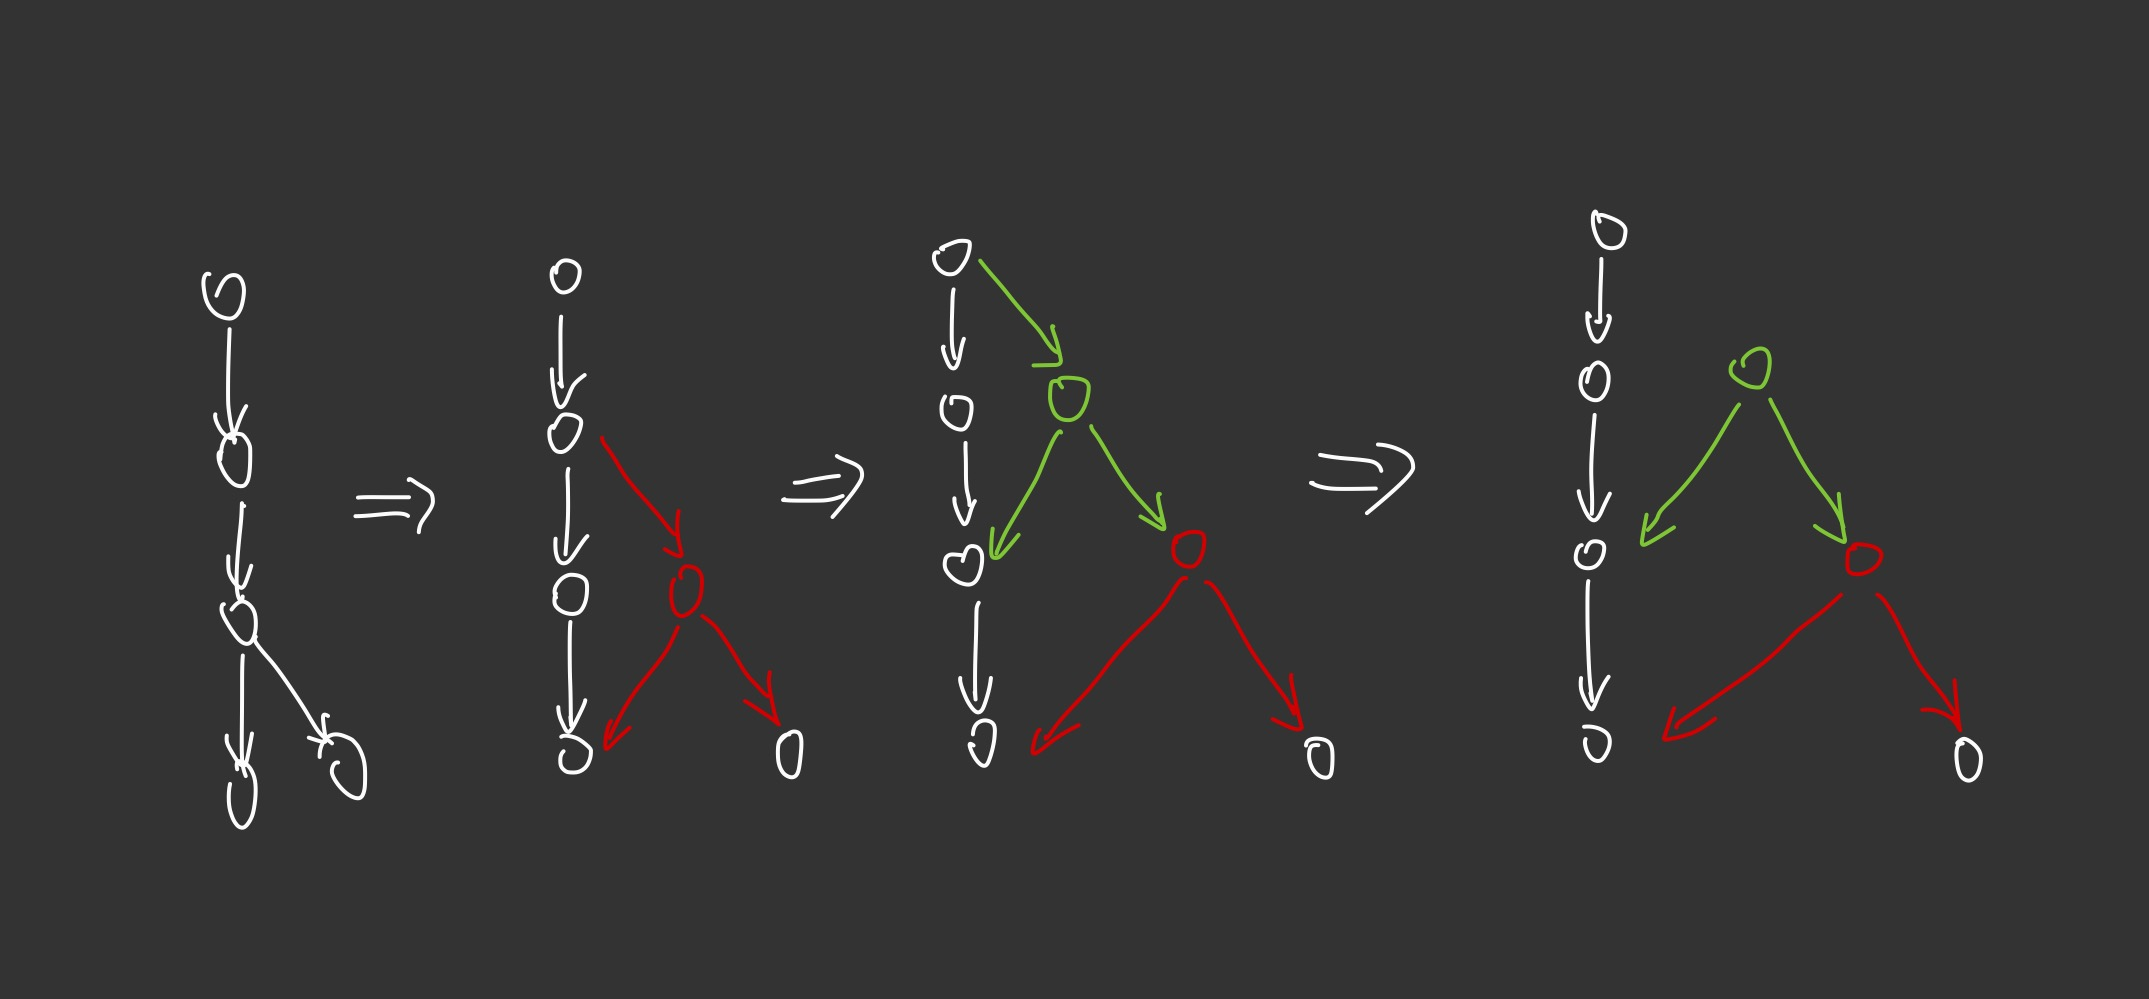
\includegraphics[width=0.8\textwidth]{images/BFE42FBF-CA3E-492F-89B4-7F5677DA8246.jpeg}
    \caption{Refinement for single path}
    \label{fig:refine3}
    \end{figure}
    可以看到这里处理的路径个数和路径的长度是关系的, 准确来说如果CFG上实际存在$n$条候选错误路径, 那么实际可能分析$O(2^n)$路径. 这个直觉来源于你如果copy一个结点,那么你就会将通过这个点的所有路径数乘2.
    \item 准确来说我们总是strengthen某个结点上的条件,这个strengthen过程就是通过新增一个conjunct再取反. i.e, $\neg (\neg \varphi_1 \wedge \varphi_2)$. 这里的直觉是什么呢? 我们知道一个predicate可以将整个程序状态空间一分为二, 满足它的状态和不满足它的状态, 对应这个predicate本身和它的取反形式. 例如当$\varphi_1$对应的状态无法reach到某个结点, 那么可能reach这个结点的状态只能在$\neg \varphi_1$中了. 接着我们分析了一条新路径在对应结点产生$\varphi_2$, 此时原本这个结点上还有一个$\neg \varphi_1$, 那么实际的条件就是$\neg \varphi_1 \wedge \varphi_2$. 可以看出来我们在$\neg \varphi_1$基础上又strengthen了一次,如果这个条件依然不行,那么再取反分割结点. 两次取反你会发现$\varphi_1$又回来了, 但是我们之前已经排除了$\varphi_1$. 这个方案告诉你取反并不是一种比较好的办法,它太弱了.
      
    我们可以直接新增一个取反的后conjunct, 不再直接取反, i.e., $\neg \varphi_1 \wedge \neg \varphi$. 这相当于就是把已经探索过的路径条件都给收集起来了.
    \item 每次只会对一个结点加annotation, 即frontier上的一段. 这样的后果就是我们得重复计算路径条件, 参考图\ref{fig:refine3}.      
\end{itemize}    
\end{example}

\begin{annotation}
\rm 前面第一个例子里面用到了给结点加label的概念, 我们可以给它形式化一下, 设label map $f_l: V_2 \to L$. 那么上面的例子中$L$为logic formulas $\mathcal{L}(\Sigma)$, 于是$G_2$上每一个结点都对应一个formula, 没有显式标注的label的结点, 都默认label为true. 后面记录两种对上述navie方法的改进:
\begin{itemize}
	\item Unfolding.
	\item Lazy annotation.
\end{itemize}
\end{annotation}

\begin{definition}
\rm Given label map $f_l: V_2 \to \mathcal{L}(\Sigma)$ of graph $G_2=(V_2,E_2)$ and $u,w \in V_2$. We say $u$ is covered by $w$, if
\begin{itemize}
	\item $f_v(u) = f_v(w)$ and 
	\item $f_l(u) \supset f_l(w)$ ($\supset$ w.r.t implies).
\end{itemize}
\end{definition}

\begin{annotation}
\rm 当label作为所在结点需要满足的状态时,$u$ is covered by $w$就意味着$w$可以reachable的结点,那么$u$也一定是可以reachable的. 按照这个思路我们就可以尝试去优化前面的分析方法. 
\end{annotation}

\begin{example}
\rm Example \ref{ex:refine_path1}中实际在划分某一结点的所有程序状态, 将不可达的程序状态都从CFG上剥离出去了.
\end{example}

\section{Model Checking}

\subsection{Bounded Model Checking}

\subsection{Interpolation and SAT-Based Model Checking}

\begin{annotation}
\rm 遵循unrolling的策略,给定一个初始状态$I_0$, check它所有$k$可达的状态. 这里我们可以利用interpolation的想法给出一个关于one-step可达状态的over-approximation, 让我们在不需要增加$k$的情况下尽可能地往前分析. 这个想法的根本是如果在某个比较大的状态集中我们的checking通过了,显然那个被盖住的真正的状态集也是safe的. 同时配合bounded model checking, 增大bounder $k$, 我们也可以消除over-approximation带来的failure checking.
\end{annotation}

\begin{procedure}[H]
\SetAlgoLined
\DontPrintSemicolon
\If{$I \wedge F$ \textup{is satisfiable}}{return \textit{true}}
$R \leftarrow I$ \;
\While{\textit{true}}{
    $M' \leftarrow (R, T, F)$ \;
    $A \leftarrow \textsc{CNF}(\textsc{Pref}_1(M'), U_1)$ \;
    $B \leftarrow \textsc{CNF}(\textsc{Suff}_0^k(M'), U_2)$ \;
    \eIf{$A \wedge B$ \textup{is satisfiable}}
    {
        \eIf{$R = I$}{return \textit{true}}{abort}
    }
    {
        Let $\Pi$ be a proof of unsatisfiability of $A \wedge B$\;
        $P \leftarrow \textsc{Itp}(\Pi, A, B)$ \;
        $R' = P\left<W/W_0\right>$\;
        \If{$\redt{R' \Rightarrow R}$}{return \textit{false}}
        $R \leftarrow R \wedge R'$
    }
}
\caption{FiniteRun({$M = (I,T,F), k > 0$})}
\end{procedure}

\begin{annotation}
\rm 上面的算法完整的描述利用interpolation在$k$-bound下做的checking,目的是找到满足某种property的状态. 其中$M=(I,T,F)$为一个target automata, $I$和$F$分布为initial state predicate和final state predicate, $T$是描述状态转移的一个predicate. SAT-based BMC的目标为
\[
    I(W_0) \wedge \left(\bigwedge_{0 \leq i < k} T(W_i, W_{i+1})\right) \wedge \left(\bigvee_{j \leq i \leq k}F(W_i)\right)
\]
是否satisfiable? 简而言之, 能否从初始状态$k$步可达的状态中找到一个满足$F$的状态. 在while之前先判断了是否存在$0$步的情况. 其中$R$表示当前所有可达的状态,初始化为$I$. 在while内,会首先创建一个new automata, 将$R$作为新的状态,去做新一轮的k-bounded checking. 这里将上面的目标分为了两个部分,前置路径和后置路径. 其中$A$表示1步前置路径
\[
    R(W_{-1}) \wedge T(W_{-1}, W_{0}),
\]
$B$表示$k$步后置路径
\[
    \left(\bigwedge_{0 \leq i \leq k} T(W_i, W_{i+1})\right) \wedge \left(\bigvee_{j \leq i \leq k}F(W_i)\right)
\]
注意这里变成了$k+1$步. 如果在第一次循环下就有$A \wedge B$ is sat, 那么这个时候checking就结束了, 因为这里的$R$此时并不是over-approximation. 反之则直接abort了, 需要重新调整$k$才行, 因为我们不能保证这里是误报还是真的counterexample. 如果$A \wedge B$ is unsat, 那么这个时候我们就可以induce出来一个interpolant $P$满足$A \to P$ and $P \wedge B$ is unsat. 接着我们需要将$P$中的prime variables变回一般的state space得到$R'$. 此时从$R'$出发的$k$步状态都是不满足$F$的, 并且从$R$出发的$k+1$步状态都是不满足$F$的. 此时的$R'$可以理解为关于$R$出发1步可达状态的一个over-approximation. 因此下一轮$R$应该为$R \vee R'$, 这个新的$R$保持了从$R$出发的$k$步状态都是不满足$F$,因此需要往后考虑一下$k+1$步. 所以这个$k$实际是限制$R'$的步长的. 最重要地是理解算法中的红色部分,如果有$R' \Rightarrow R$, 那么$R$就是一个inductive invariant. 这是因为$I \Rightarrow R$是trivial的,再根据$R \wedge T \to R'$ ($R'$ is interpolant),显然有$R \wedge T \to R$. 当$R$是一个inductive invariant的时候,再配合$R \wedge F$ is unsat, 可以知道所有reachable states都是不满足$F$, 我们的checking也结束了.

上面实际更像更像$k+1$ BMC. 我们来考虑一下细节,先考虑直接划分$k$ BMC得到A, B
\[
   \underbrace{I(W_0) \wedge T(W_0, W_1)}_{A} \wedge \underbrace{\left(\bigwedge_{0<i<k} T(W_i, W_{i+1}) \right) \wedge \left(\bigvee_{j \leq i \leq k}F(W_i)\right)}_B
\]
假设$C$是关于$A \wedge B$一个interpolant. 到底应该如何理解$C$是个什么呢? 问题的关键是$A$和$B$实际呈现是什么东西. $A$应该是characterize从初始状态一步可达状态,这样$A \to C$就意味着从初始状态一步可达状态都满足$C$. 而$B$应该是characteriz从$k-1$可达最终状态($\neg P$)的状态, 这样$C \wedge B$ is unsat就意味着满足$C$的状态都至少不能在$k-1$步到底最终状态. 
\end{annotation}

\subsection{IC3}

\begin{annotation}
\rm IC3的核心就是strengthening property直到inductive或者遇到反例无法用unreachability剔除. 这种想法把常规的abstraction和refinement过程糅杂地不那么明显了. 比较难理解是clauses传递过程, 正确的视角是把一个clause当做一个predicate,整个IC3依然是在predicate abstraction的范畴下. “向前传递”实际上对应了post operation, 而新增clause实际是在refine原本的abstract model消除反例. 

对于一个给定的transition system $S:(\overline{x}, I, T)$和一个safety property $P$. 整个过程将构造一串formulas $F_0 = I,F_1,F_2,\cdots,F_k$表示对应$0, 1, \cdots, k$可达状态的over-approximation,它们满足下述性质:
\begin{enumerate}
    \item $I \Rightarrow F_0$;
    \item $F_i \Rightarrow F_{i+1}$ for $0 \leq i < k$;
    \item $F_i \Rightarrow P$ for $0 \leq i \leq k$;
    \item $F_i \wedge T \Rightarrow F'_{i+1}$ \footnote{这里是$F'_{i+1}$而不是$F_{i+1}$, 如果写成后者, 这里就会与(2)出现歧义. $F'_{i+1}$表示将$F_{i+1}$中的variables $\{x_i\} $都换成带prime的variables $\{x_i'\}$} for $0 \leq i < k$ .
\end{enumerate}
一旦出现$\textup{clauses}(F_i) = \textup{clauses}(F_{i+1})$,那么$F_i$就是我们要找的那个strengthening clauses such that $F_i \wedge P \wedge T \Rightarrow F_i \wedge P$.

接下来看看这串$F_i$是如何构造的. 
\begin{itemize}
    \item Base case: check the satisfiability of $I \wedge \neg P$ ($I \Rightarrow P$ is true e.q. to $I \wedge \neg P$ is unsat) and $I \wedge T \wedge \neg P'$. 这是对$0$-step和$1$-step的一个check.
    \item Inductive case: 当$k > 0$时,假设$F_0,F_1,\cdots,F_k$满足上述4个性质. 现在来尝试构造$F_{k+1}$. 首先check $F_k \wedge T \Rightarrow P'$是否存在.
    \begin{itemize}
        \item 如果$F_k \wedge T \Rightarrow P'$. 此时让$F_{k+1} = P$, 显然当前sequence依然保持上述4个性质. 另外还要做一个操作,将$F_0, F_1, \cdots, F_k$中的clauses ``向前移动": 对于任意$c \in F_i$ ($0 \leq i \leq k$), 如果$F_i \wedge T \Rightarrow c'$并且$c \notin \textup{clauses}(F_{k+1})$, 那么让$F_{k+1} \leftarrow F_{k+1} \wedge c$. 如果这个操作过程中发现存在$\textup{clauses}(F_i) = \textup{clauses}(F_{i+1})$,那么找到了strengthening clauses $F_i$.
        \item 如果$F_k \wedge T \nRightarrow P'$. 那么这里一定存在一个state $s \models F_k$使得它的下一个状态并不满足$P$. 这里下一步的做法就是尝试把$s$剔除,就是要证明$s$是unreachable. 也就是证明$\neg s$是inductive invariant. 首先确定$0\leq i \leq k$中最大的$i$使得$\neg s$ is inductive relative to $F_i$,即$i \Rightarrow \neg s$ and $F_i \wedge \neg s \Rightarrow \neg s$. 如果这样的$i$不存在,即$\neg s$ is not even inductive relative to $F_0$, 那么显然$s$就无法排除了, 这就意味着$P$ is not inductive invariant. 如果这样的$i$存在,再对$s$做一次inductive generalization, 找到mininal subclause $c \subseteq \neg s$ that is inductive relative to $F_i$. 接着将$c$作为一个conjunct依次放到$F_0, \cdots, F_{i+1}$上. 首先把$c$放到$F_0, \cdots,F_i$上并不会违反上述四个性质, 这一点很容易check. 其次最后是$F_{i+1}$,这是因为$F_{i} \wedge \neg s \wedge T \Rightarrow \neg s'$, 配合性质(4), 可以得到$F_{i} \wedge \neg s \wedge T \Rightarrow F_{i+1}' \wedge \neg s'$. 
        
        如果$i \geq k - 1$, 显然$s$已经被排除在$F_k$. 比较难处理的是$i < k-1$的情况, 此时并没有把$s$从$F_k$中去掉. 这里需要先思考一下为什么$\neg s$会是在$F_i$上inductive而不是$F_{i+1}$? 这里可以形式化一下这个问题:
        \[
            \begin{aligned}
            F_{i+1} \wedge \neg s \wedge T \nRightarrow \neg s \\
            F_{i} \wedge \neg s \wedge T \Rightarrow \neg s \\
            \end{aligned}
        \]
        那么这里必然存在一个状态$t$满足
        \[
            t \models F_{i+1} ~\textup{and}~ t \not\models F_{i}~\textup{and}~(t,s) \in T.
        \]
        也就是说存在一个$F_{i+1}$中的状态$t$,它下一个状态满足$s$. 如果能将这样的$t$从$F_{i+1}$都剔除去,那么也会有$\neg s$ is inductive relative to $F_{i+1}$. 现在的目标就是让$\neg t$ is inductive relative to $F_{i}$ (注意这里不是$i+1$), 和前面对$s$的处理是高度重合的. 但这里有一个好的性质是当$i > 0$时, $\neg t$至少在$F_{i-1}$是inductive的. 这是因为根据前面的条件,这里有$F_{i} \Rightarrow \neg t$, 所以这里的难度小于对$s$的处理. 接着我们继续考虑使用这样的方法处理$i+2, i+3,\cdots, k$, 最终$\neg s$会在$F_{k-1}$上inductive,这样就把$s$从$F_k$中剔除了. 我们又回到了考虑$F_k \wedge T \Rightarrow P'$的情况. 
        
        现在我们的条件应该是这样的
        \[
            \left\{
            \begin{aligned}
                &s \models F_k \\
                &(s,u) \in T \\
                &u \not\models P
            \end{aligned} \right.
        \]
        确定一个小claim: \redt{当$k > 2$时,$\neg s$ is inductive relative to $F_{k-2}$}. 假设$\neg s$ is not inductive relative to $F_{k-2}$, 则
        \[
            F_{k-2} \wedge \neg s \wedge T \Rightarrow s.
        \]
        再配合一下性质(4), 显然我们得到
        \[
            F_{k-2} \wedge \neg s \wedge T \Rightarrow s \wedge F_{k-1}
        \]
        这就意味着$s$也在$F_{k-1}$中,这和$F_{k-1} \wedge T \Rightarrow P$是矛盾的. 上面这个claim意味着我们找那个最大值$i$似乎也不太麻烦, 甚至有点一击必中的感觉. 
    \end{itemize}
\end{itemize}
\end{annotation}


\begin{annotation}
\rm 我觉得比较好的理解IC3的顺序应该是先看看understanding IC3, 理解里面介绍的incremental construction是什么,再看看IC3之前的作者另一个工作FSIS里面的inductive generalization思想. 最后再来主攻IC3.
\end{annotation}

\newpage
\section{Martain L\"{o}f Type Theory}

\subsection{Universe and Families}

\begin{definition}
\rm A \redt{universe} is type whose elements are types.
\end{definition}

\begin{annotation}
\rm 为了避免Russell's paradox在集合论中尴尬,可以定义一组分层的universe:
\[
	\mathcal{U}_0 : \mathcal{U}_0 :\mathcal{U}_2 : \cdots
\]
其中每一个$\mathcal{U}_i$是$\mathcal{U}_{i+1}$中的元素. 同样允许当$A:\mathcal{U}_i$, 也有$A : \mathcal{U}_{i+1}$. 但是这里可能有一个小问题就是这样使得$A$的类型不唯一了. 当某个$\mathcal{U}$被确定了之后,它包含的types通常称为\redt{small types}.
\end{annotation}

\begin{definition}
\rm Given type $A$, the functions $B: A \to \mathcal{U}$ whose codomain is a universe are called \redt{families of type} $A$.
\end{definition}

\begin{annotation}
\rm family是一个比较重要的component, 它用于描述a collection of types varying over a given type $A$.
\end{annotation}

\begin{example}\label{ex:family_fin}
\rm 设$\text{Fin}:\mathbb{N} \to \mathcal{U}$, 其结果表示恰好只存在$n$个元素它们的类型为$\text{Fin}(n)$, 也就是说"满足" $\text{Fin}(n)$的元素只有$n$个, 即$0_{n}: \text{Fin}(n), 1_{n}: \text{Fin}(n), \cdots, (n-1)_n : \text{Fin}(n)$. 给出一个agdastdlib里面的构造
\[
    \begin{aligned}
    &\text{zero} : \text{Fin}~(\text{suc}~n) \\
    &\text{suc}  : (i : \text{Fin}~n) → \text{Fin} ~(\text{suc}~n)
    \end{aligned}
\]
每个type $\text{Fin}~n$都有一元素$\text{zero}$, 而对于每一个$i_{n} : \text{Fin}~(n)$都可以得到一个$i_{n+1} : \text{Fin}~(n+1)$.
\end{example}


\begin{example}
\rm 一个constant type family 为 $B:\mathcal{U}$. 
\end{example}

\subsection{Dependent Function Types(\texorpdfstring{$\Pi$}{pi}-types)}


\begin{definition}
\rm Given a type $A:\mathcal{U}$ and a family $B:A \to \mathcal{U}$, then $\Pi_{(x:A)} B(x):\mathcal{U}$ is type of dependent functions whose domain is element $x$ of type $A$ and  codomain is element of type $B(x)$. There is a alternative notation for this type, such as $\Pi(x : A).B(x)$.
\end{definition}

\begin{annotation}
\rm dependent funtion和type family的区别是什么? 前者的函数输出 (function result) 为一个term,后者的输出是一个type.
\end{annotation}


%https://math.stackexchange.com/questions/2007230/whats-the-difference-between-a-dependent-function-type-pi-types-and-a
\begin{example}
\rm 取\ref{ex:family_fin}中的family $\text{Fin}:\mathbb{N} \to \mathcal{U}$, 我们可以构造一个dependent function $\text{Fmax}:\Pi_{n : \mathbb{N}} \text{Fin}(n+1)$, 其结果表示非空集合$\text{Fin}(n+1)$中"最大值" (或者说最后一个元素) , 即$\text{Fmax}(n) \defeqv n_{(n+1)}$\footnote{$\defeqv$表示function definition} 
\end{example}

\begin{example}
\rm 当family $B$是一个constant family时,有$\Pi_{(x:A)} B(x) \equiv A \to B$\footnote{$\equiv$表示definitional equality}, 即non-dependent function type. 这也说明dependent function type是一种general form.
\end{example}

\begin{example}
\rm 如果一个dependent function接受一个type作为参数,此时我们可以称它为polymorphic function, 例如polymorphic identity function $\text{id}:\Pi_{A:\mathcal{U}} A \to A$.
\end{example}

\begin{example}
\rm 如果一个dependent functuon同样可以接受多个参数,例如polymorphic swap function $\text{swap}: \Pi_{A:\mathcal{U}}\Pi_{B:\mathcal{U}}\Pi_{C:\mathcal{U}}(A \to B \to C) \to (B \to A \to C)$, 它对应的function definition为
\[
	\text{swap}(A,B,C,g) \defeqv \lam{b}{\lam{a}{g(a)(b)}}.
\]
swap可以用来交换function里面两个arguments.
\end{example}

\subsection{Dependent Pair Types}

\begin{annotation}
\rm 这里有一个uniqueness principle,可以简单地理解为先用一次introduction rule构造$a : A$, 再用一次elimination rule给$a : A$"拆开", 然后再用一次introduction rule我们又可以得到$a : A$. 例如给定$x : A \times B$, 那么它的uniqueness principle 就是$(\pi_1(x), \pi_2(x)) \equiv x$ . 注意这是一个命题, 它表示所有$x : A \times B$, 其$x$都是一个ordered pair, 所以了这个definitional equality是需要证明的,因此也可以叫做propositional uniqueness principle. 
\end{annotation}

\begin{annotation}
\rm 另外一个需要说明的是这里我们并没有规定product type就必须是一个pair, 也就是说这个东西并没有作为规则写到type theory中. 当然你要是说introductionl rule里面似乎已经规定了, 那确实是,但是需要证明.
\end{annotation}

\begin{definition}
\rm 对于任意的function $g: A \to B \to C$, 我们都可以定义一个function $f: A \times B \to C$使得
\[
	f((a,b)) \defeqv g(a)(b)
\]
$f$ is well-defined when we specify its values on pairs.
\end{definition}

\begin{definition}
\rm Two projection functions:
\[
	\begin{aligned}
	\pi_1: A \times B \to A \\
	\pi_2: A \times B \to B
	\end{aligned}
\]
其中
\[
	\begin{aligned}
	\pi_1((a,b)) \defeqv a \\
	\pi_2((a,b)) \defeqv b 
	\end{aligned}
\]
\end{definition}

\begin{annotation}
上面两个projections中的$g_1 : A \to B \to A$和$g_2: A \to B \to B$分别为
\[
    \begin{aligned}
    g_1 \defeqv \lam{x}{\lam{y}{x}} \\
    g_1 \defeqv \lam{x}{\lam{y}{y}}
    \end{aligned}
\]
\end{annotation}

\begin{definition}
\rm Given a product type $A \times B$. Define function $\text{rec}_{A \times B}$ as the recursor for $A \times B$ with type
\[
	\text{rec}_{A \times B}:\Pi_{C:\mathcal{U}}(A \to B \to C) \to A \times B \to C
\]
and defining equation
\[
	\text{rec}_{A \times B}(C, g, (a,b)) \defeqv g(a)(b).
\]
\end{definition}

\begin{example}
\rm 此时我们可以用$\text{rec}_{A \times B}$来定义$\pi_1$和$\pi_2$:
\[
	\begin{aligned}
	\pi_1 \defeqv \text{rec}_{A \times B}(A, \lam{a}{\lam{b}{a}}) \\
	\pi_2 \defeqv \text{rec}_{A \times B}(B, \lam{a}{\lam{b}{b}})
	\end{aligned}
\]
有一个比较特殊的nullary product type $\mathbf{1}$, 它只有一个inhabitant我们可以用$\star:\mathbf{1}$表示. 它也有一个对应的recursor $\text{rec}_\mathbf{1}: \Pi_{C:\mathcal{U}} C \to \mathbf{1} \to C$, 它的defining equation为
\[
	\text{rec}_\mathbf{1}(C, c, \star) \defeqv c 
\]
这是因为你从$\mathbf{1}$中不能获取任何信息.

可以看到recursion实际是一个更为general elimination rule (The recursion pinciple for catesian products is the fact that we can define a function $f:A \times B \to C$ as above by giving its value on pairs).
\end{example}

\begin{annotation}
\rm 关于product types的dependent functions $f: \Pi_{x:A\times B}C(x)$, 其中$C: (A \times B) \to \mathcal{U}$. 我们也使用一个elimination rule: 给定任意的function $g:\Pi_{x:A}\Pi_{y:B}C((x,y))$, 我们可以定义dependent function $f: \Pi_{x:A\times B}C(x)$.
\[
	f((x,y)) \defeqv g(x)(y).
\]
\end{annotation}

\begin{definition}
\rm A judgmental equality or definitional equality is the notion of equality which is defined to be a judgement, we write it as $a \equiv b : A$ or simply $a \equiv b$.
\end{definition}

\begin{definition}
\rm A proposition equality is a proposition, so it is also a type such that $a =_A b$, and to prove the proposition is to find term of type $a =_A b$.
\end{definition}

\begin{example}
\rm 现在我们来证明product type只能是一个pair, 我们尝试构造这样一个dependent function $\text{uniq}_{A \times B}:\Pi_{x:A \times B}((\pi_1(x),\pi_2(x)) =_{A \times B} x)$, 通过defining equation
\[
	\text{uniq}_{A \times B}((a,b)) \defeqv \text{refl}_{(a,b)}.
\]
其中$\text{refl}_{x}: x =_A x$ for any $x:A$是一个well-typed element. 那么$C(x) \equiv (\pi_1(x),\pi_2(x)) =_{A \times B} x)$, 那么当$x \defeqv (a,b)$, 我们可以得到
\[
	C(x) \defeqv (\pi_1(((a,b)),\pi_2((a,b))) =_{A \times B} (a,b)
\]
显然有
\[
	(\pi_1(((a,b)),\pi_2((a,b))) \equiv (a,b)
\]
因此$\text{refl}_{(a,b)}: (\pi_1(((a,b)),\pi_2((a,b))) = (a,b)$还是well-typed. 所以关于$\text{uniq}_{A \times B}$整个构造是对的,如何进一步说明$x$确实是一个pair呢? 难度从$f$是well-defined? 推出其所有结果都是well-typed, 然后$x$ is equal to a pair.
\end{example}


\begin{annotation}
\rm 如果你把前面的dependent function $f$当做一个predicate来描述所有类型为product type的元素的某种property,同时把(ordered) pair当做product type的canonical element. 那么就意味$f$只需要作用到这些canonical elements上就够了, 这样就可以导出induction.
\end{annotation}

\begin{definition}
\rm Given a product type $A \times B$. Define a function $\text{ind}$ as the induction for $A \times B$ with the type
\[
	\text{ind}_{A \times B}: {\Pi}_{C:A \times B \to \mathcal{U}}(\Pi_{x:A}\Pi_{y:A} C((x,y))) \to \Pi_{x:A\times B} C(x)
\]
and the defining equation:
\[
	\text{ind}_{A \times B}(C, g, (a,b)) \defeqv g(a)(b).
\]
\end{definition}

\begin{annotation}
\rm 这个就是更加general的elimination rule了,如果前面的recursion rule叫做non-dependent eliminator, 那么这个induction就可以叫做dependent eliminator.
\end{annotation}

\begin{example}
\rm 关于unit type $\mathbf{1}$的induction为
\[
    \text{ind}_\mathbf{1}: \Pi_{C:\mathbf{1} \to \mathcal{U}} C(\star) \to \Pi_{x:\mathbf{1}} C(x)
\]
with the defining equation
\[
    \text{ind}_\mathbf{1}(C,c,\star) \defeqv c.
\]
通过$\text{ind}_\mathbf{1}$我们也可以知道unit type只有对应的一个元素,这就是unit type的uniqueness principle. 因为我们构造一个dependent function
\[
    \text{uniq}_1:\Pi_{x:\mathbf{1}} x=\star
\]
with defining equation
\[
    \text{uniq}_\mathbf{1} \defeqv \text{ind}_\mathbf{1}(\lam{x}{x = \star}, \text{refl}_\star)
\]
\end{example}

\begin{definition}
\rm Given a type $A:\mathcal{U}$ and a family $B: A \to \mathcal{U}$, the dependent pair type is written as $\sum_{(x:A)} B(x)$.
\end{definition}

\begin{example}
\rm 当$B$是一个constant的时候, 此时$\Sigma_{(x:A)} B$就是product type.
\end{example}

\begin{definition}
\rm Given a function $g:\Pi_{x:A} B(x) \to C$, we can define a function out of a $\Sigma$-type $f:(\Sigma_{x:A}B(x)) \to C$ via the defing equation
\[
    f((a,b)) = g(a)(b)
\]
\end{definition}

\begin{example}
\rm 关于$\Sigma$-type两个non-dependent projection function定义如下: the first projection function
\[
    \pi_1:(\Sigma_{x:A}B(x)) \to A
\]
with the defining equation
\[
    \pi_1((a,b)) \defeqv a.
\]
The second projection function
\[
    \pi_2:\Pi_{p:(\Sigma_{x:A}B(x))} B(\pi_1(p)) 
\]
这里我们还无法构造$\pi_2$,因为我们还不知道$\Sigma$-type的dependent function如何构造.
\end{example}

\begin{definition}
\rm Given a function $g:\Pi_{a:A}\Pi_{b:B(a)} C((a,b))$, we can define a dependent function $f: \Pi_{p:\Sigma_{x:A} B(x)} C(p)$ with defining equation
\[
    f((a,b)) \defeqv g(a)(b)
\]
\end{definition}

\begin{definition}
\rm The induction for $\Sigma$-type $\Sigma_{x:A}B(x)$ is 
\[ 
    \text{ind}_{\Sigma_{x:A}B(x)}: \Pi_{C:(\Sigma_{x:A}B(x) \to \mathcal{U})}(\Pi_{a:A}\Pi_{b:B(a)} C((a,b))) \to \Pi_{p:(\Sigma_{x:A}B(x))} C(p) 
\]
with defining equation.
\[
    \text{ind}_{\Sigma_{x:A}B(x)} (C, g, (a,b)) \defeqv g(a)(b)
\]
\end{definition}

\begin{example}
\rm Assume $R : A \to B \to \mathcal{U}$, then type-theoretic axiom of choice is
\[
    \text{ac}: \Pi_{x : A}\Sigma_{y : B} R(x,y) \to \Sigma_{f : A \to B} \Pi_{x: A} R(x, f(x))
\]
with defining equation
\[
    \text{ac} (g) \defeqv (\lam{x}{\pi_1(g(x))}, \lam{x}{\pi_2(g(x))}).    
\]
将$\Pi$看做$\forall$, 而将$\Sigma$看做$\exists$, 就比较好理解了.
\end{example}

\subsection{Coproduct Type}

\begin{definition}
\rm A coproduct type is formed as $A + B$ with introductions rules
\[
    \infer[+\textsc{Intro}_1]{\text{inl}(a) : A + B}{a : A}  \quad \infer[+\textsc{Intro}_2]{\text{inr}(b) : A + B}{b : A}
\]
\end{definition}

\begin{definition}
\rm The recursion principle of coproduct type is
\[
    \text{rec}_{A + B} : \Pi_{C : \mathcal{U}} (A \to C) \to (B \to C) \to A + B \to C
\]
with defining equation
\[
    \begin{aligned}
    \text{rec}_{A + B}(C, g_0, g_1, \text{inl}(a)) \defeqv g_0(a) \\
    \text{rec}_{A + B}(C, g_0, g_1, \text{inr}(b)) \defeqv g_1(b) 
    \end{aligned}
\]
where $g_0 : A \to C$ and $g_1 : B \to C$.
\end{definition}

\begin{definition}
\rm The induction principle of coproduct type is
\[
    \text{ind}_{A + B} : \Pi_{C : A + B \to \mathcal{U}} (\Pi_{x : A} C(\text{inl}(x))) \to (\Pi_{y : B} C(\text{inr}(y))) \to \Pi_{z : A + B} C(z)
\]
with defining equation
\[
    \begin{aligned}
    \text{ind}_{A + B}(C, g_0, g_1, \text{inl}(a)) \defeqv g_0(a) \\
    \text{ind}_{A + B}(C, g_0, g_1, \text{inr}(b)) \defeqv g_1(b) 
    \end{aligned}
\]
where $g_0 : \Pi_{x : A} C(\text{inl}(x))$ and $g_1 : \Pi_{y : A} C(\text{inr}(y))$. 
\end{definition}


\subsection{Concrete Construction}

\begin{definition}
\rm The constructors for $\mathbb{N}$ are
\[
    \begin{aligned}
        &0 : \mathbb{N} \\
        &\text{succ} : \mathbb{N} \to \mathbb{N} 
    \end{aligned}
\]
\end{definition}

\begin{definition}
\rm Primitive recursion of $\mathbb{N}$ is 
\[
    \begin{aligned}
    &f(0) \defeqv c_0 \\
    &f(\text{succ}~n) \defeqv c_s(n, f(n))
    \end{aligned}
\]
where $f: \mathbb{N} \to C$, $c_0 :\mathbb{N}$ and $c_s : \mathbb{N} \to C \to C$.
\end{definition}

\begin{annotation}
\rm 注意上面用到了primitive这个词,它意味着这个recursion可以盖住所有$f: \mathbb{N} \to C$的构造. 如果想要构造$\mathbb{N}$上的加法, 我们只需要这个$C$换成$N \to N$, 那么此时$c_0 : \mathbb{N} \to \mathbb{N}$, 而$c_s : \mathbb{N} \to (\mathbb{N} \to \mathbb{N}) \to (\mathbb{N} \to \mathbb{N})$. 此时$f$我们用$\text{add}$来表示,那么$\text{add}(n)$实际就是plus operator $n+$, $\text{add(0)} \defeqv c_0$表示即$0+$, 而$\text{add}(\text{succ}~n) = c_s(n, add(n))$表示$n+1+$.
\end{annotation}

\begin{definition}
\rm Recursor of $\mathbb{N}$ is
\[
    \text{rec}_{\mathbb{N}} : \Pi_{C : \mathcal{U}} \to C \to (\mathbb{N} \to C \to C) \to \mathbb{N} \to C
\]
with defining equation
\[
    \begin{aligned}
        &\text{rec}_{\mathbb{N}}(C, c_0, c_s, 0) \defeqv c_0 \\
        &\text{rec}_{\mathbb{N}}(C, c_0, c_s, \text{succ}~n) \defeqv c_s(n,  \text{rec}_{\mathbb{N}}(C, c_0, c_s, n))
    \end{aligned}
\]
\end{definition}

\begin{definition}
\rm Induction principle of $\mathbb{N}$ is 
\[
    \text{ind}_{\mathbb{N}} : \Pi_{C : \mathbb{N} \to \mathcal{U}} C(0) \to (\Pi_{n : \mathbb{N}} C(n) \to C(\text{succ}~n)) \to \Pi_{n: N} C(n)
\]
with defining equation
\[
    \begin{aligned}
        &\text{ind}_{\mathbb{N}}(C, c_0, c_s, 0) \defeqv c_0 \\
        &\text{ind}_{\mathbb{N}}(C, c_0, c_s, \text{succ}~n) \defeqv c_s(n,  \text{ind}_{\mathbb{N}}(C, c_0, c_s, n))
    \end{aligned}
\]
\end{definition}

\subsection{Programming Language Definition}

\begin{annotation}
\rm Given the type $\Sigma_{x : A} P(x)$, we can regard it as the type of all elements $x : A$ such that $P(x)$.
\end{annotation}

\subsection{Algebraic Structure Definition}

\begin{example}
\rm A type of magma is 
\[
    \text{Magma} : \Sigma_{A : \mathcal{U}} A \to A \to A.
\]
Magma可以刻画那些带有binary operator的代数结构. 其中$A$实际就代表了a set of elements, 我们可以通过$\pi_1$拿到. 而其binary operator, 我们可以通过$\pi_2$拿到.
\end{example}

\begin{example}
\rm A type of pointed-magma is 
\[
    \text{PointedMagma} : \Sigma_{A : \mathcal{U}} (A \to A \to A) \times A.
\]
相比于Magmas, 这里多出了一些点$x : A$, 例如我们常常需要的identity element.
\end{example}

\begin{example}
\rm A type of boolean is $\mathbf{2} : \mathcal{U}$ is intended to have exactly two elements $0_{2}, 1_2 : \mathbf{2}$. 我们可以用coproduct type配合unit type来定义它, i.e., $\mathbf{1} + \mathbf{1}$, 这里就正好有两个元素. 当然了也可以显式地直接定义$\mathbf{2}$.

依赖boolean type的if-then-else对应的recursion principle为
\[
    \text{rec}_{\mathbf{2}} : \Pi_{C : \mathcal{U}} C \to C \to \mathbf{2} \to C 
\]
with defining equation
\[
    \begin{aligned}
    \text{rec}_{\mathbf{2}}(C, c_0, c_1, 0_2) = c_0 \\
    \text{rec}_{\mathbf{2}}(C, c_0, c_1, 1_2) = c_1  
    \end{aligned}
\]
\end{example}

\subsection{Identity Types}

\begin{definition}
\rm Given two elements $a b : A$, there is type $a =_A b : \mathcal{U}$ called \emph{identity type} or \emph{equality type} in the same universe.
\end{definition}

\begin{definition}
\rm The only introduction rule for identity types is a dependent function
\[
    \refl : \Pi_{a : A} (a =_A a)
\]
called \redt{reflexivity}.
\end{definition}

\begin{definition}
\rm (\redt{Indiscernibility of identicals}) For every family $C : A \to \mathcal{U}$, there is a function
\[
    f: \Pi_{x,y : A} \Pi_{p : x =_A y} ~C(x) \to C(y)
\]
such that $f(x,x,\refl_x) \defeqv \id_C(x)$.
\end{definition}

\begin{annotation}
\rm Indiscernibility of identicals描述当两个东西是相同的时候, 当其中一个满足某种性质的时候,另外一个也应当满足这个性质. 在任何使用它们的场景下都是无法区分它们的.
\end{annotation}

\begin{lemma}
\rm (\redt{Principle of substitution}) To prove that every $x,y$ with $x = y$ has property $P(x,y)$, it suffices to prove that every pair $x,x$ (for which $x = x$) has property $P(x,x)$
\end{lemma}

\begin{proof}
By Indiscernibility of identicals for $x = y$, we know $P(x,x) \to P(x,y)$ (fixed the first argument).
\end{proof}

\begin{annotation}
\rm MLTT中也有一个类似path induction的identify type的elimination rule.
\end{annotation}

\newpage
\section{Homotopy Type Theory}
\begin{annotation}
Topologically, ...
\end{annotation}

\begin{definition}
\rm Topologically, a identity type is a \redt{path}.  
\end{definition}

\subsection{Path Induction}
\begin{annotation}
\rm \redt{The family of identity types is freely generated by the reflexivity terms}.
\end{annotation}

\begin{definition}
\rm (\redt{Path induction}) Given a family $C : \Pi_{x,y : A} (x =_A y) \to \mathcal{U}$ and a function $c : \Pi_{x : A} C(x, x, \refl_x)$, there is a function 
\[
    f : \Pi_{x,y : A} \Pi_{p : x =_A y} C(x,y,p)
\]
such that $f(x,x,\refl_x) \defeqv c(x)$. It corresponds a single function
\[
    \ind_{=A} : \Pi_{C : \Pi_{x, y : A} (x =_A y) \to \mathcal{U}}~ (\Pi_{x : A} C(x,x,\refl_x)) \to \Pi_{x, y : A} \Pi_{p : x=_A y} C(x,y,p)
\]
with the equality $\ind_{=A}(C,c,x,x,\refl_x) \defeqv c(x)$.
\end{definition}

\begin{annotation}
\rm Given a identity type family $C$, to prove that every pair $x,y$ with path $p : x = y$ has property $C(x,y,p)$, it suffices to prove that every pair $x,x$ with loop $\refl_x$ has property $C(x,x,\refl_x)$. 
\end{annotation}

\begin{annotation}
\rm 辅助理解path induction, 思考$1 + 3 = 3 + 1$的证明过程. 这里应该有一些类似的证明, 例如
\[
\begin{aligned}
    1 + 3 = 0 + 4 = 4 = 4 = 1 + 3 = 2 + 2 = 3 + 1 \\
\end{aligned}
\]
但是无论怎样我们都无法直接用$\refl_{1+3}$或者$\refl_{3+1}$来一步到位,而是连续地使用了$\refl$. 这里看起来identity type是inductive defined, 注意这并不对! 这里$1 + 3 = 3 + 1$是一个non-dependent identity type family $C(x,y,p) \defeqv 1 + 3 = 3 + 1$, 因此还是identity type family是inductive defined. 可以更general一点,来证明 $1 + x = x + 1$, 我们也可以借助identity type,构造一个family $C(x, y, p) \defeqv 1 + x = y + 1$.
\end{annotation}

\begin{definition}
\rm (\redt{Based path induction}) Fix an element $a :A$, we have a dependent function
\[
    \ind_{=A}' : \Pi_{a : A} \Pi_{C : \Pi_{x : A} (a =_A x) \to \mathcal{U}}~  C(a,\refl_a) \to \Pi_{x : A} \Pi_{p : a=_A x} C(x, p) 
\]
with the equality 
\[
    \ind_{=A}'(a, C, c, a,  \refl_a) \defeqv c.
\]
\end{definition}

\begin{annotation}
\rm 注意这里不能同时固定$x,y : A$. 特别地,换句话说我们不能只通过$C(\refl_x)$来证明$C(p)$ with $p : x =_A x$. 因为HoTT允许$x, x$之间的paths不只有reflexivity.

从拓扑的观点来看,一个两端固定的绳子可能不能连续形变到同一个点 (constant path (路径只在某一点上)). 例如给定挖掉圆心的圆 $\{(x,y) | 0 < x^2 + y^2 < 2\}$. 我们来考虑两种情况
\begin{center}
    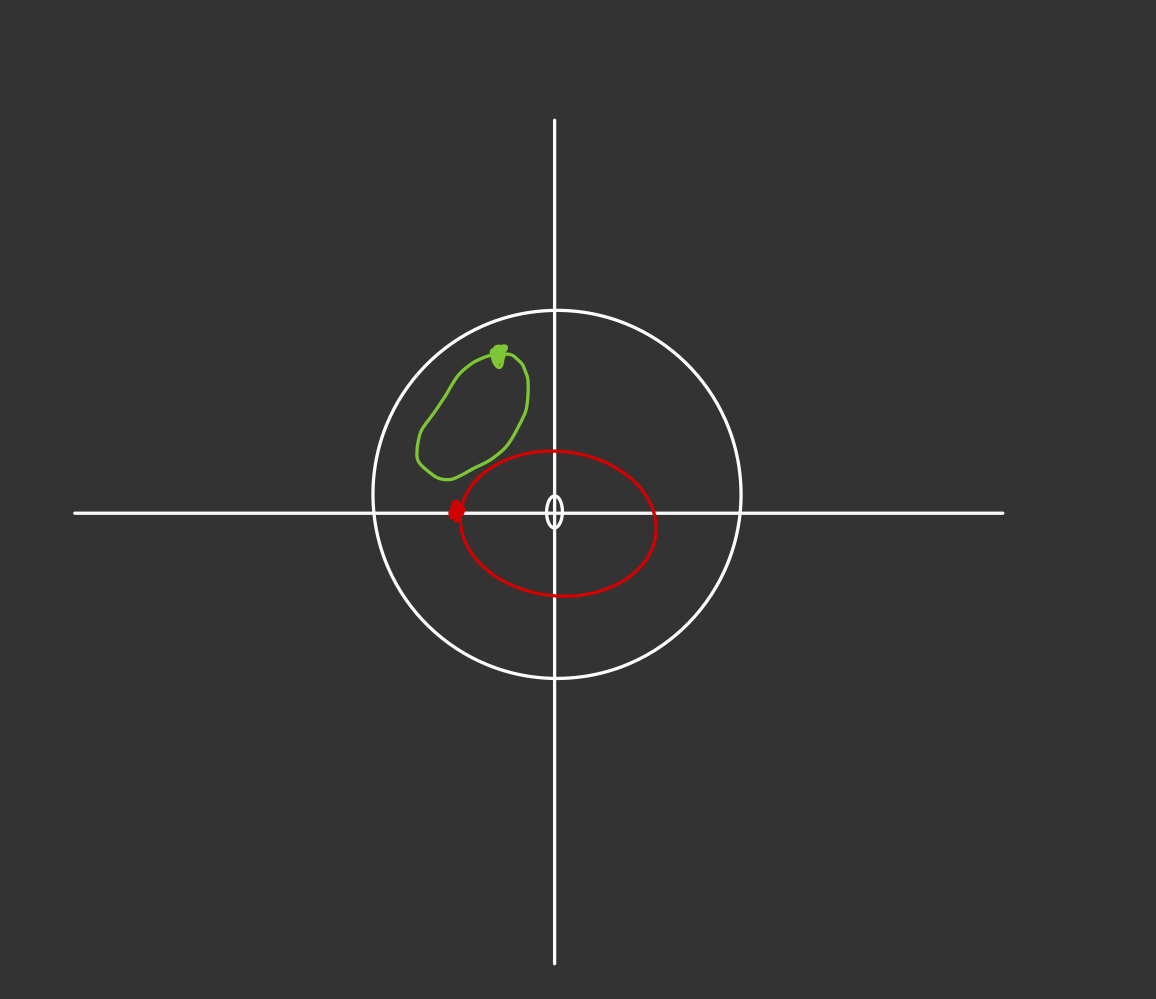
\includegraphics[scale=0.1]{images/topo1.png}
\end{center}
绿色的环显然是可以连续形变到这个环上的某个点, 但是红色的环不行. 因为中间的这个洞阻碍了连续形变. 如果运行这个环的某个端点可变,显然我们可以一直收缩这个端点到另外一个端点. 连续形变相当于在其过程中产生了很多的paths, 这些paths都是"连续"的或者homotopical.
\end{annotation}

\begin{lemma}
\rm Path induction and based path induction are equivalent.
\end{lemma}

\begin{proof}
($\Leftarrow$)是简单的,即
\[
    \begin{aligned}
     \text{eq}_l : &(\ind_2 :(\Pi_{a : A} \Pi_{C : \Pi_{x : A} (a =_A x) \to \mathcal{U}}~  C(a,\refl_a) \to \Pi_{x : A} \Pi_{p : a=_A x} C(x, p))) \\ 
     \to&(\ind_1 : (\Pi_{C : \Pi_{x, y : A} (x =_A y) \to \mathcal{U}}~ (\Pi_{x : A} C(x,x,\refl_x)) \to \Pi_{x, y : A} \Pi_{p : x=_A y} C(x,y,p)))
    \end{aligned}
\]
with the equality $\text{eq}_l(\ind_2, C, c, x, y, p) = \ind_2(x, C(x), c(x), y, p)$.

反过来就有点不太明显了, 即要证
\[
    \begin{aligned}
     \text{eq}_r : &(\ind_1 : (\Pi_{C : \Pi_{x, y : A} (x =_A y) \to \mathcal{U}}~ (\Pi_{x : A} C(x,x,\refl_x)) \to \Pi_{x, y : A} \Pi_{p : x=_A y} C(x,y,p)))  \\
     \to&(\ind_2 :(\Pi_{a : A} \Pi_{C : \Pi_{x : A} (a =_A x) \to \mathcal{U}}~  C(a,\refl_a) \to \Pi_{x : A} \Pi_{p : a=_A x} C(x, p)))
    \end{aligned}
\]
这个时候没法直接用$\ind_1$. 这里我们需要利用path induction去额外证明一个property
\[
    f : \Pi_{x,y : A} \Pi_{p : x = y} \Pi_{C : \Pi_{z : A} (x =_A z) \to \mathcal{U}} ~ C(x,\refl_x) \to C(y,p).
\]
使得$D : \Pi_{x, y : A} (x = y) \to \mathcal{U}$ with $D(x, y, p) = \Pi_{C : \Pi_{z : A} (x =_A z) \to \mathcal{U}} C(x,\refl_x) \to C(y,p)$. 这里$D$就是$x = y$的一个family, 我们可以利用path induction来证明
\[
    f : \Pi_{x,y : A} \Pi_{p : x = y} D(x,y,p) 
\]
显然有$D(x,x,\refl_x) = \id_{C(x,\refl_x)}$. 因此我们有$\text{eq}_r(\ind_2, a, C, c, x, p) = f(a, x, p, C, c)$. 

这里还需要注意是如果$\text{eq}_r$里面规定$C : \Pi_{x : A} (a = x) \to \mathcal{U}_i$, 那么必须需要$D : \Pi_{x, y : A} (x = y) \to \mathcal{U}_{i+1}$.  因为$D$的参数是$c : C$, 由此可能会产生类型为$\mathcal{U}_i$的元素,盖住它们需要用更高一层的universe.
\end{proof}

\begin{annotation}
\rm 如何使用path induction呢? 也就是说如何用path induction证明一些function $f$ ?

如果我们type family $D : \Pi_{x,y : A} (x = y) \to \mathcal{U}$和$d : \Pi_{a:A} D(a,a,\refl_a)$,那么我们就可以得到一个dependent function
\[
    \ind_{=A}(D,d) : \Pi_{x,y:A}\Pi_{p : x = y} D(x,y,p)
\]
with the definition equality $\ind_{=A}(D,d,a,a,\refl_a) \defeqv d(a)$. 

首先$f$应当是关于every $x,y$ with $p : x=y$的一个proprety, 此时就可以用$D$来抽象这个property. 并且$D(x,y,p)$应当是描述property中结果的那个type. 有可能此时$D(x,x,\refl)$还需要继续用path induction, 也就是无法直接构造$d$. 在下面一个小节中可以慢慢体会这个过程.
\end{annotation}


\subsection{Types are higher groupoids}

\begin{lemma}
\rm For every type $A$ and every $x,y : A$ there is a function
\[
    (x = y) \to (y = x)
\]
denoted $p \mapsto p^{-1}$, such that $\refl_x^{-1} \equiv \refl_x$ for each $x : A$. We call $p^{-1}$ the \redt{inverse} of $p$.
\end{lemma}

\begin{proof}
\rm The corresponding type for the proposition is
\[
    f : \Pi_{A : \mathcal{U}} \Pi_{x , y : A} (x = y) \to (y = x).
\]
Let $D : \Pi_{x, y : A} (x = y) \to \mathcal{U}$ be the type family defined by $D(x,y,p) \defeqv (y=x)$. Then we have an element $d \defeqv \lam{x}{\refl_x} : \Pi_{x : A} D(x,x,\refl_x)$. Thus, the induction principle for identity types gives us an element $\ind_{=A}(D,d,x,y,p) : (y = x)$.
\end{proof}

\begin{lemma}
\rm For every type $A$ and every $x,y,z : A$ there is a function 
\[
    (x = y) \to (y=z) \to (x=z)
\]
written $p \mapsto q \mapsto p \centerdot q$, such that $\refl_x \centerdot \refl_x \equiv \refl_x$ for any $x : A$. We call $p \centerdot q$ the \redt{concatenation} or \redt{composite} of $p$ and $q$.
\end{lemma}

\begin{proof}
\rm The corresponding type for the proposition is
\[
    \Pi_{A : \mathcal{U}}\Pi_{x,y,z : A} ~ (x = y) \to (y=z) \to (x=z)
\]
Let $D_1 : \Pi_{x,y} (x=y) \to \mathcal{U}$ be the family defined by $D_1(x,y,p) \equiv \Pi_{z : A} \Pi_{q : y = z} (x=z)$. Now $D(x,x,\refl_x) = \Pi_{z : A}\Pi_{q : x = z} (x=z)$. Let $D_2 : \Pi_{x,z : A} \Pi_{q : x=z}~\mathcal{U}$ be the family defined by $D_2(x,z,q) \defeqv x = z$. Now $D_2(x,x,\refl_x) \equiv (x=x)$, then we have $d_2 : \Pi_{x:A} ~ D_2(x,x,\refl_x)$ defined by $d_2(x) = \refl_x$. 

By induction principle for identity type we have $\ind_{=A} (D_2,d_2) : \Pi_{x,z : A} \Pi_{p : x=z} x = z$. Then we have $d_1 : \Pi_{x : A} D_1(x,x,\refl)$ defined by $d_1(x) = \ind_{=A} (D_2,d_2)$. Again by induction principle for identity type we have $\ind_{=A} (D_1,d_1) : \Pi_{x,y : A} \Pi_{p : x=y} \Pi_{z : A} \Pi_{q : y = z} (x=z)$. Since $p$ and $q$ is unused, then $\ind_{=A} (D_1,d_1) : \Pi_{x,y : A} (x=y)  \to \Pi_{z : A} (y = z) \to (x=z)$. Finally we have $\ind_{=A} (D_1,d_1) : \Pi_{x,y,z : A} (x=y)  \to (y = z) \to (x=z)$.
\end{proof}

\begin{definition}
\rm A $\infty$-groupoid consists of a collection of objects, and then a collection of morphisms between objects, and then morphisms between morphisms, and so on. Morphisms at each level have identity, composition, and inverse operations.
\end{definition}

\begin{remark}
\rm “equality”, “homotopical”, and “higher-groupoid” points of view on what we have done so far. 
\begin{center}
    \begin{tabular}{|c|c|c|}
     \hline Equality & Homotopy & $\infty$-Groupoid \\
     \hline reflexivity & constant path & identity morphism \\
     \hline symmetry & inversion of paths & inverse morphism \\
     \hline transitivity & concatenation of paths & composition of morphisms \\
     \hline
\end{tabular}
\end{center}
\end{remark}

\begin{lemma}
\rm (\redt{2-path}) Suppose $A :\mathcal{U}$, that $x, y, z, w : A$ and that $p : x = y$ and $r : z = w$. We have the following:
\begin{itemize}
    \item $p = p \centerdot \refl_y$ and $p = \refl_x \centerdot p$.
    \item $p^{-1} \centerdot p = \refl_y$ and $p \centerdot p^{-1} = \refl_x$.
    \item $(p^{-1})^{-1} = p$.
    \item $p \centerdot (q \centerdot r) = (p \centerdot q) \centerdot r$.
\end{itemize}
\end{lemma}

\begin{proof}
我们在这里只证明associativity.  它对应的type为
\[
    \Pi_{x,y,z,w : A} \Pi_{p : x=y} \Pi_{q : y = z} \Pi_{r : z = w} ~ p \centerdot (q \centerdot r) = (p \centerdot q) \centerdot r
\]
使得$D_1 : \Pi_{x,y : A} \Pi_{p : x=y}~\mathcal{U}$ defined by 
\[
    D_1(x,y,p) =\Pi_{z}\Pi_{q : y=z}\Pi_{w : A} \Pi_{r : z = w} ~ p \centerdot (q \centerdot r) = (p \centerdot q) \centerdot r
\]
此时$D_1(x,x,\refl_x) = \Pi_{z, w : A}\Pi_{q : x = z}\Pi_{r : z = w}~\refl_x \centerdot (q \centerdot r) = (\refl_x \centerdot q) \centerdot r$.

再使得$D_2 : \Pi_{x, z : A} \Pi_{q : x=z} \to \mathcal{U}$ defined by 
\[
    D_2(x,z,q) = \Pi_{w : A}\Pi_{r : z = w} ~\refl_x \centerdot (q \centerdot r) = (\refl_x \centerdot q) \centerdot r.
\]
此时$D_2(x,x,\refl_x) = \Pi_{w : A}\Pi_{r : x = w } ~\refl_x \centerdot (\refl_x \centerdot r) = (\refl_x \centerdot \refl_x) \centerdot r$.

最后使得$D_3 : \Pi_{x, w : A} \Pi_{r : x = w } \mathcal{U}$ defined by
\[
    D_3(x, w, r) = \refl_x \centerdot (\refl_x \centerdot r) = (\refl_x \centerdot \refl_x) \centerdot r
\]
此时$D_3(x,x,\refl_x) = \refl_x \centerdot (\refl_x \centerdot \refl_x) = (\refl_x \centerdot \refl_x) \centerdot \refl_x$. 因此$d_3 : \Pi_{x} D_3(x,x,\refl_x)$ defined by $d_3(x) = \refl_{\refl_x}$, 注意这里是2-path.

最后用两次path induction,构造$d_2$和$d_1$, 和一次path induction证明原命题. 
\end{proof}

\begin{lemma}
\rm (\redt{Right whiskering}) Suppose $a, b : A$ and $p, q : a = b$ and $\alpha : p = q$ and $r : b = c$, then we can define
\[
    a \centerdot_r r : p \centerdot r = q \centerdot r
\]
\end{lemma}

\begin{proof}
By induction on $r$, it suffices to assume $r$ as $\refl_b$, then $a \centerdot_r \refl : p \centerdot \refl_b = q \centerdot \refl_b$ can be defined by
\[
    a \centerdot_r \refl_b \defeqv {\textbf{ru}_p}^{-1} \alpha \textbf{ru}_q 
\]
where $\textbf{ru}_p : p = p \centerdot \refl_b$ and $\textbf{ru}_q : q = q \centerdot \refl_b$. 
\end{proof}

\begin{lemma}
\rm (\redt{Left whiskering}) Suppose $b, c : A$ and $r, s : b = c$ and $\beta : r = s$ and $q : a = b$, then we define
\[
    q \centerdot_l \beta : q \centerdot r = q \centerdot s
\]
\end{lemma}

\begin{annotation}
\rm 前面两个whiskering lemma告诉我们2-path可以直接concact相同path的, 来产生一个新的2-path, 这就带来了一些等号上好的计算性质. 
\end{annotation}

\begin{lemma}
\rm (\redt{Horizontal composition}) Suppose $a,b,c : A$ and $p,q: a = b$ and $r,s : b = c$ and $\alpha : p = q$ and $\beta : r = s$. Then we can define
\[
    \alpha \star \beta : p \centerdot r = q \centerdot s
\]
\begin{center}
    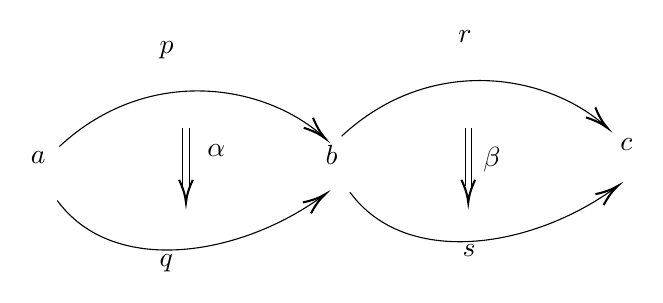
\begin{tikzpicture}[x=0.75pt,y=0.75pt,yscale=-1,xscale=1]
%uncomment if require: \path (0,497); %set diagram left start at 0, and has height of 497

%Curve Lines [id:da4580105282751987] 
\draw    (136,369) .. controls (155.75,396.06) and (194.22,397.98) .. (229.12,385.32) .. controls (241.35,380.88) and (253.15,374.65) .. (263.54,367.08) ;
\draw [shift={(265,366)}, rotate = 143.13] [color={rgb, 255:red, 0; green, 0; blue, 0 }  ][line width=0.75]    (10.93,-3.29) .. controls (6.95,-1.4) and (3.31,-0.3) .. (0,0) .. controls (3.31,0.3) and (6.95,1.4) .. (10.93,3.29)   ;
%Curve Lines [id:da6945510671526884] 
\draw    (137,343) .. controls (179.36,303.6) and (235.29,312.71) .. (263.72,337.84) ;
\draw [shift={(265,339)}, rotate = 222.88] [color={rgb, 255:red, 0; green, 0; blue, 0 }  ][line width=0.75]    (10.93,-3.29) .. controls (6.95,-1.4) and (3.31,-0.3) .. (0,0) .. controls (3.31,0.3) and (6.95,1.4) .. (10.93,3.29)   ;
%Curve Lines [id:da19013021837951216] 
\draw    (273,338) .. controls (315.36,298.6) and (371.29,307.71) .. (399.72,332.84) ;
\draw [shift={(401,334)}, rotate = 222.88] [color={rgb, 255:red, 0; green, 0; blue, 0 }  ][line width=0.75]    (10.93,-3.29) .. controls (6.95,-1.4) and (3.31,-0.3) .. (0,0) .. controls (3.31,0.3) and (6.95,1.4) .. (10.93,3.29)   ;
%Curve Lines [id:da5521038491120764] 
\draw    (277,365) .. controls (303.73,401.63) and (364.76,392.2) .. (404.79,362.89) ;
\draw [shift={(406,362)}, rotate = 143.13] [color={rgb, 255:red, 0; green, 0; blue, 0 }  ][line width=0.75]    (10.93,-3.29) .. controls (6.95,-1.4) and (3.31,-0.3) .. (0,0) .. controls (3.31,0.3) and (6.95,1.4) .. (10.93,3.29)   ;
%Straight Lines [id:da951832554297978] 
\draw    (199.5,334) -- (199.5,362)(196.5,334) -- (196.5,362) ;
\draw [shift={(198,370)}, rotate = 270] [color={rgb, 255:red, 0; green, 0; blue, 0 }  ][line width=0.75]    (10.93,-3.29) .. controls (6.95,-1.4) and (3.31,-0.3) .. (0,0) .. controls (3.31,0.3) and (6.95,1.4) .. (10.93,3.29)   ;
%Straight Lines [id:da620936274617875] 
\draw    (335.5,334) -- (335.5,362)(332.5,334) -- (332.5,362) ;
\draw [shift={(334,370)}, rotate = 270] [color={rgb, 255:red, 0; green, 0; blue, 0 }  ][line width=0.75]    (10.93,-3.29) .. controls (6.95,-1.4) and (3.31,-0.3) .. (0,0) .. controls (3.31,0.3) and (6.95,1.4) .. (10.93,3.29)   ;

% Text Node
\draw (122,344) node [anchor=north west][inner sep=0.75pt]    {$a$};
% Text Node
\draw (264,341) node [anchor=north west][inner sep=0.75pt]    {$b$};
% Text Node
\draw (406,338) node [anchor=north west][inner sep=0.75pt]    {$c$};
% Text Node
\draw (184,291) node [anchor=north west][inner sep=0.75pt]    {$p$};
% Text Node
\draw (328,286) node [anchor=north west][inner sep=0.75pt]    {$r$};
% Text Node
\draw (184,394) node [anchor=north west][inner sep=0.75pt]    {$q$};
% Text Node
\draw (330,389) node [anchor=north west][inner sep=0.75pt]    {$s$};
% Text Node
\draw (207,341) node [anchor=north west][inner sep=0.75pt]    {$\alpha$};
% Text Node
\draw (340,342) node [anchor=north west][inner sep=0.75pt]    {$\beta$};


\end{tikzpicture}
\end{center}
\end{lemma}

\begin{proof}
\rm We can define $\alpha \star \beta : p \centerdot r = q \centerdot s$ by
\[
    \alpha \star \beta \defeqv (\beta \centerdot_r r) \centerdot (q \centerdot_l \beta).
\]
\end{proof}


\begin{definition}
\rm A \redt{pointed type} $(A, a)$ is a type $A : \mathcal{U}$ together with a point $a : A$, called its basepoint.We write $\mathcal{U}_{\bullet}\defeqv \Sigma_{A : \mathcal{U}} A$ for the type of pointed types in the universe $\mathcal{U}$.
\end{definition}

\begin{definition}
\rm Given a pointed type $(A, a)$, we define the \redt{loop space} of $(A, a)$ to be following pointed type:
\[
    \Omega(A, a) \defeqv ((a =_A a), \refl_a).
\]
An element of it will be called a \redt{loop} at $a$. For $n : \mathbb{N}$, the $n$-fold iterated loop space $\Omega^{n}(A, a)$ of a pointed type $(A, a)$ is defined recursively by:
\[
    \begin{aligned}
        \Omega^0(A, a) &\defeqv (A, a) \\
        \Omega^{n+1}(A, a) &\defeqv \Omega^n(\Omega(A,a)).
    \end{aligned}
\]
An element of it will be called an $n$-loop or an $n$-dimensional loop at $a$.
\end{definition}

\begin{annotation}
\rm Loop space可以看做所有点$a$上loops, 这样的loops可以用$a =_A a$来表示,特别地有一个特殊的loop叫做$\refl_a$. 
\end{annotation}

\subsection{Functions are Functors}

\begin{lemma}
\rm Suppose that $f : A \to B$ is a function. Then for any $x,y : A$ there is an operation
\[
    \ap_f:(x =_A y) \to (f(x) =_B f(y)).
\]
Moreover, for each $x : A$ we have $\ap_f(\refl_x) \equiv \refl_{f(x)}$. We often write $f(p)$ as $\ap_f(p)$.
\end{lemma}

\begin{annotation}
\rm $\ap_f$可以看做the application of $f$ to a path or the action on paths of $f$.
\end{annotation}


\begin{lemma}
\rm For functions $f : A \to B$ and $g : B \to C$ and paths $p : x=_A y$ and $q : y=_A z$, we have
\begin{itemize}
    \item Functoriality : $\ap_f(p \centerdot q) = \ap_f(p)\centerdot \ap_f(q)$.
    \item Reflectivity : $\ap_f(p^{-1}) = \ap_f(p)^{-1}$.
    \item Functor composition : $\ap_g(\ap_f(p)) = \ap_{g \circ f}(p)$.
    \item Identity functor : $\ap_{\id_A}(p) = p$.
\end{itemize}
\end{lemma}

\subsection{Type Families are Fibrations}

\begin{annotation}
\rm 如果给定一个dependent function $f : \Pi_{x : A} B(x)$ 和 $p : x = y$, 那么我们是否可以直接构造$f(x) = f(y)$ ? 显然不行,因为$B(x)$和$B(y)$可能并不是同一个类型. 所以这里有一些gap, 这些gap可以通过探究$p$本身蕴含的一些东西来解决. 
\end{annotation}

\begin{lemma}
\rm (\redt{Transport}) Suppose that $P$ is a type family over $A$ and that $p : x =_A y$. Then there is a function $p_*: P(x) \to P(y)$. We often write $\transport^P(p,-) : P(x) \to P(y)$.
\end{lemma}

\begin{proof}
\rm The corresponding type is
\[
    f : \Pi_{P : A \to \mathcal{U}}\Pi_{x,y : A} (x=y) \to (P(x) \to P(y)).
\]
By induction, it suffices to assume $p$ is $\refl_x$, then $f(P, x,x,\refl_x) = \refl_{P(x)}$.
\end{proof}

\begin{proof}
\rm 这个$\transport$和indistinguiability of identicals实际上一样的,都在说如果$x = y$,那么$P(x)$成立当且仅当$P(y)$成立, 其中$P$可以看做关于type $A$的一个property. 

从拓扑的观点来看,可以将$P : A \to \mathcal{U}$看做 a \redt{fibration} with base space $A$, with P(x) being the fiber over x, and with $\Sigma_{x : A} P(x)$ being the \redt{total space} of the fibration, with first projection $\Sigma_{x : A} P(x) \to A$. 如果存在$u : P(x)$, 那么path $p : x = y$ 就可以对应total space中的一个path $(x, u) = (y, p_*(x)))$. 这个过程称为path lifting.
\begin{center}
    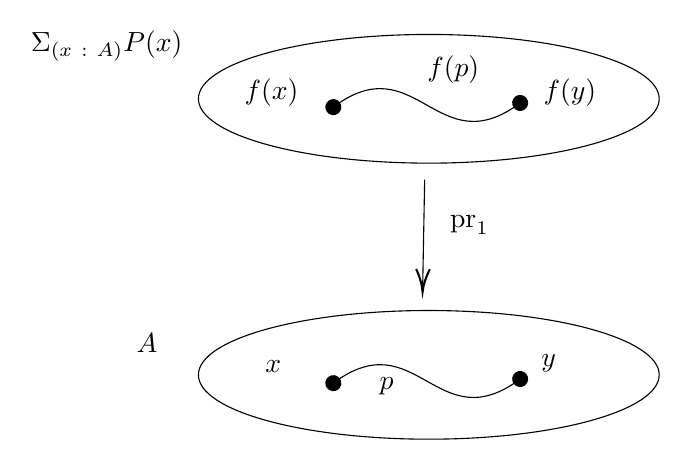
\begin{tikzpicture}[x=0.75pt,y=0.75pt,yscale=-1,xscale=1]
%uncomment if require: \path (0,300); %set diagram left start at 0, and has height of 300

%Shape: Ellipse [id:dp8188930674915369] 
\draw   (170,71) .. controls (170,53.88) and (219.7,40) .. (281,40) .. controls (342.3,40) and (392,53.88) .. (392,71) .. controls (392,88.12) and (342.3,102) .. (281,102) .. controls (219.7,102) and (170,88.12) .. (170,71) -- cycle ;
%Curve Lines [id:da7500318047279952] 
\draw    (235,75) .. controls (275,45) and (285,103) .. (325,73) ;
\draw [shift={(325,73)}, rotate = 323.13] [color={rgb, 255:red, 0; green, 0; blue, 0 }  ][fill={rgb, 255:red, 0; green, 0; blue, 0 }  ][line width=0.75]      (0, 0) circle [x radius= 3.35, y radius= 3.35]   ;
\draw [shift={(235,75)}, rotate = 323.13] [color={rgb, 255:red, 0; green, 0; blue, 0 }  ][fill={rgb, 255:red, 0; green, 0; blue, 0 }  ][line width=0.75]      (0, 0) circle [x radius= 3.35, y radius= 3.35]   ;
%Shape: Ellipse [id:dp5278439924527563] 
\draw   (170,204) .. controls (170,186.88) and (219.7,173) .. (281,173) .. controls (342.3,173) and (392,186.88) .. (392,204) .. controls (392,221.12) and (342.3,235) .. (281,235) .. controls (219.7,235) and (170,221.12) .. (170,204) -- cycle ;
%Curve Lines [id:da6542980978586372] 
\draw    (235,208) .. controls (275,178) and (285,236) .. (325,206) ;
\draw [shift={(325,206)}, rotate = 323.13] [color={rgb, 255:red, 0; green, 0; blue, 0 }  ][fill={rgb, 255:red, 0; green, 0; blue, 0 }  ][line width=0.75]      (0, 0) circle [x radius= 3.35, y radius= 3.35]   ;
\draw [shift={(235,208)}, rotate = 323.13] [color={rgb, 255:red, 0; green, 0; blue, 0 }  ][fill={rgb, 255:red, 0; green, 0; blue, 0 }  ][line width=0.75]      (0, 0) circle [x radius= 3.35, y radius= 3.35]   ;
%Straight Lines [id:da31936463691040573] 
\draw    (279,110) -- (278.04,162) ;
\draw [shift={(278,164)}, rotate = 271.06] [color={rgb, 255:red, 0; green, 0; blue, 0 }  ][line width=0.75]    (10.93,-3.29) .. controls (6.95,-1.4) and (3.31,-0.3) .. (0,0) .. controls (3.31,0.3) and (6.95,1.4) .. (10.93,3.29)   ;

% Text Node
\draw (191,60) node [anchor=north west][inner sep=0.75pt]    {$f( x)$};
% Text Node
\draw (335,60) node [anchor=north west][inner sep=0.75pt]    {$f( y)$};
% Text Node
\draw (279,49) node [anchor=north west][inner sep=0.75pt]    {$f( p)$};
% Text Node
\draw (201,196) node [anchor=north west][inner sep=0.75pt]    {$x$};
% Text Node
\draw (334,193) node [anchor=north west][inner sep=0.75pt]    {$y$};
% Text Node
\draw (256,204) node [anchor=north west][inner sep=0.75pt]    {$p$};
% Text Node
\draw (290,126) node [anchor=north west][inner sep=0.75pt]    {$\text{pr}_{1}$};
% Text Node
\draw (139,183) node [anchor=north west][inner sep=0.75pt]    {$A$};
% Text Node
\draw (88,37) node [anchor=north west][inner sep=0.75pt]    {$\Sigma _{( x\ :\ A)} P( x)$};


\end{tikzpicture}
\end{center}
\end{proof}

\begin{lemma}
\rm (\redt{Path lifting property}). Let $P : A \to \mathcal{U}$ be a type family over $A$ and assume we have $u : P(x)$ for some $x : A$. Then for any $p : x=y$, we have
\[
    \lift(u,p) : (x, u) = (y, p_*(x)).
\]
in $\Sigma_{x : A} P(x)$, such that $\pr_1(\lift(u,p)) = p$.
\end{lemma}

\begin{definition}
\rm Given a type family $P : A \to \mathcal{U}$, a dependent function $f : \Pi_{x :A} P(x)$ is a \redt{section} of the fibration $P$. If such $f$ is exists, we say there is \redt{fiberwise} happened.
\end{definition}

\begin{annotation}
\rm 在给定一个section $f : \Pi_{x :A} P(x)$的情况下, 我们可以定义一个non-dependent function $f' : A \to \Sigma_{x : A} P(x)$ defined by $f'(x) \defeqv (x, f(x))$. 这样我们再把$\ap$用在$f'$上了,那么$f'(p) : f'(x) = f'(y)$. 但是type $f'(x) = f'(y)$并不能很好的显示这个total space上path是基于哪个$p : x=y$的, 也就是我们希望$p$也出现最后我们得到的那个equality type中. 于是就有下面的定义. 
\end{annotation}

\begin{lemma}
\rm (\redt{Dependent map}) Suppose $f : \Pi_{x : A} P(x)$, then we have a map
\[
  \apd_f : \Pi_{p : x = y} (p_*(f(x))) =_{P(y)} f(y))  
\]
\end{lemma}

\begin{proof}
\rm By induction, it suffices to assume $p$ is $\refl_x$, then $\apd_f(\refl_x) = \refl_{f(x)}$. 
\end{proof}

\begin{annotation}
\rm 我们让$u : P(x)$和$v : P(y)$, 那么$p_*(u) = v $就可以看做"a path form $u$ to $v$ lying over $p : x=y$". 
\end{annotation}

\begin{lemma}
\rm (\redt{Constantly transport}) If $P : A \to \mathcal{U}$ is defined by $P(x) \defeqv B$ for a fixed $B : \mathcal{U}$, then for any $x, y : A$ and $p : x=y$ and $b : B$ we have a path
\[
    \transportconst_p^B(b) : \transport^P(p, b) = b.
\]
\end{lemma}

\begin{annotation}
\rm 有了$\transportconst$之后, 对应任意的$x,y : A$, $p : x = y$和$f : A \to B$, 我们可以构造一个function
\[
    \text{eq}_1 : f(x) = f(y) \to p_*(f(x)) = f(y)
\]
with definition equality
\[
    \text{eq}_1(\ap_f(p)) = \transportconst_p^B(f(x)) \centerdot \ap_f(p). 
\]
反过来,我们可以用$\transportconst^{-1}$来构造function
\[
    \text{eq}_2 : p_*(f(x)) = f(y) \to f(x) = f(y)
\]
with definition equality
\[
    \text{eq}_2(\apd_f(p)) =  {\transportconst_p^B}^{-1}(f(x)) \centerdot \apd_f(p). 
\]
接着我们可以证明$\text{eq}_1(\ap_f(p)) = \apd_f(p)$.
\end{annotation}

\newpage
\subsection{Homotopies and Equivalences}

\begin{definition}
\rm Let $f, g : \Pi_{x : A} P(x)$ be two sections of a type family $P: A \to \mathcal{U}$. A \redt{homotopy} from $f$ to $g$ is a dependent function of type
\[
    (f \sim g) \defeqv \Pi_{x : A} (f(x) = g(x)).
\]
\end{definition}

\begin{annotation}
\rm 一个homotopy $f \sim g$可以从几个方面来理解:
\begin{itemize}
    \item 可以看做是由很多continous paths $f(x) = f(y)$构成的.
    \item 把$f,g$看做两个functors, 那么$f \sim g$是一个natural transformation.
\end{itemize}
\end{annotation}

\begin{lemma}
\rm Homotopy is an equivalent relation on each dependent function type $\Pi_{x:A} P(x)$.
\end{lemma}

\begin{lemma}
\rm (\redt{Natural transformation}) Suppose $H : f \sim g$ is a homotopy between dependent functions $f,g: \Pi_{x:A} P(x)$ and let $p : x=y$. Then we have 
\[
    H(x) \centerdot g(p) = f(p) \centerdot H(y).
\]
That is below diagram is commutative
\begin{center}
% https://tikzcd.yichuanshen.de/#N4Igdg9gJgpgziAXAbVABwnAlgFyxMJZABgBpiBdUkANwEMAbAVxiRADMAKADwEoQAvqXSZc+QigDM5KrUYs2XAJ78hI7HgJEyk2fWatEIAOY9VwkBg3ii03dX0KjplYNkwox+EVDsAThAAtkhkIDgQSACMDvKGHJxo-NQMdABGMAwACqKaEiAMMOw4INQAFjB0UGyQYKzJWLVsUBBMqQWCFv5BIdThSABMMQZsABJmJflpGdnWWkZ+WMalxWUVVUY1dfkNcc2t7WocAcGI0WERiNJyw0ZjrslTWTk2RgVFE+WV1QRbDDtNLTarEOXROg3OSCujjipkSExS6SeszyCyWKxAn3W4B+8P+Rj2QLcAiAA
\begin{tikzcd}
f(x) \arrow[rrr, "f(p)", Rightarrow, no head] \arrow[ddd, "H(x)"', Rightarrow, no head] &  &  & f(y) \arrow[ddd, "H(y)", Rightarrow, no head] \\
                                                                                        &  &  &                                               \\
                                                                                        &  &  &                                               \\
g(x) \arrow[rrr, "g(p)"', Rightarrow, no head]                                          &  &  & g(y)                                         
\end{tikzcd}
\end{center}
\end{lemma}

\begin{proof}
\rm By induction, it suffices to assume $p$ is $\refl_x$, then $H(x) \centerdot \refl_{g(x)} = \refl_{f(x)} \centerdot H(x)$, which both sides are $H(x)$.
\end{proof}

\begin{corollary}
\rm Let $H : f \sim \id_A$ be a homotopy, with $f : A \to A$. Then for any $x : A$ we have 
\[
    H(f(x)) = f(H(x)).
\]
Here $f(x)$ denotes the ordinary application of $f$ to $x$, while $f(H(x))$ denotes $\ap_f(H(x))$.
\end{corollary}

\begin{proof}
\rm We know $H(x) : f(x) = x$, let $p$ be $H(x)$. By naturality of $H$, we have following commutative diagram:
\begin{center}
% https://tikzcd.yichuanshen.de/#N4Igdg9gJgpgziAXAbVABwnAlgFyxMJZABgBpiBdUkANwEMAbAVxiRADMAKLgDwEo+IAL6l0mXPkIoAzOSq1GLNr0Eix2PASJlp8+s1aIOnfsNEgMGyUVm7q+pUZ7D5MKAHN4RUOwBOEAFskMhAcCCQARntFQ2MACRMBEGoGOgAjGAYABXFNKRAGGHYcZJAACxg6KDZIMFYUrDq2KAgmNMKzH38gxBCwpAAmaIM2BJVBFPTMnKstI18sdzKS6gqqmoJ6gsbYlraOtQ5uyOp+xFkFEaME00mM7NzrI0Li0oYd5tb21kO-QMHTuFzsNHCAbhMClMHrN8gslitypVqkZalt3k0jHtvi4hEA
\begin{tikzcd}
f(f(x)) \arrow[rrr, "f(H(x))", Rightarrow, no head] \arrow[ddd, "H(f(x))"', Rightarrow, no head] &  &  & f(x) \arrow[ddd, "H(x)", Rightarrow, no head] \\
                                                                                                 &  &  &                                      \\
                                                                                                 &  &  &                                      \\
f(x) \arrow[rrr, "H(x)"', Rightarrow, no head]                                                   &  &  & x                                   
\end{tikzcd}
\end{center}
This is $f(H(x)) \centerdot H(x) = H(f(x)) \centerdot H(x)$. We can whisker by ${H(x)}^{-1}$ to cancel $H(x)$, obtaining
\[
    f(H(x)) = f(H(x)) \centerdot H(x) \centerdot {H(x)}^{-1} = H(f(x)) \centerdot H(x) \centerdot {H(x)}^{-1} = H(f(x)).
\]
\end{proof}


\begin{definition}
\rm For a function $f : A \to B$, a \redt{quasi-inverse} of $f$ is a triple $(g, \alpha,\beta)$ consisting of a function $g : B \to A$ and homotopies $\alpha : f \circ g \sim \id_B$ and $\beta : g \circ f \sim \id_A$. We often use $\qinv(f)$ to denote the type:
\[
    \qinv(f) \equiv \Sigma_{g : B \to A}((f \circ g \sim \id_B) \times (g \circ f \sim \id_A)).
\]
\end{definition}

\begin{example}
\rm For any $p :  x=_A y $ and $z : A$, the function
\[
    (p \centerdot -) : (y =_A z) \to (x =_A z)
\]
has a quasi-inverse given by $(p^{-1} \centerdot -) : (x =_A z) \to (y =_A z)$. 

如何理解这个例子呢? 首先得把它们两个definition先给出来. 这里我们让$\textbf{concact} : \Pi_{A : \mathcal{U}}\Pi_{x,y,z : A} ~ (x = y) \to (y=z) \to (x=z)$. 那么这里有
\[
    \begin{aligned}
        (p , - ) &\defeqv \textbf{concact}(A,x,y,z,p) \\
        (p^{-1}, -) &\defeqv \textbf{concact}(A,y,x,z,p^{-1})
    \end{aligned}
\]
那么接着来考虑它们的composition
\[
    \begin{aligned}
        (p , - ) \circ (p^{-1} , -) (r) \equiv \textbf{concact}(A,x,y,z,p, \textbf{concact}(A,y,x,z,p^{-1},r))
    \end{aligned}
\]
其中$r : x =_A z$. 再接下来需要证明
\[
    \textbf{concact}(A,x,y,z,p, \textbf{concact}(A,y,x,z,p^{-1},r)) = r
\]
通过path induction, 我们证明存在一个$\refl_{x=_A x}$对应上述类型.
\end{example}


\newpage
\begin{thebibliography}{9}
\bibitem{ITLTS}
Introduction to labelled transition systems. \newline\url{http://wiki.di.uminho.pt/twiki/pub/Education/MFES1617/AC/AC1617-2-LTS.pdf}

\bibitem{AITBAC}
An Introduction to Bisimulation and Coinduction. \newline\url{https://homes.cs.washington.edu/~djg/msr_russia2012/sangiorgi.pdf}

\bibitem{mLTS}
Labelled transition systems. \newline\url{https://www.mcrl2.org/web/user_manual/articles/lts.html}


\bibitem{CCS}
A Calculus of Communicating Systems. Robin Milner. 

\bibitem{BMGM15}
Baluda, Mauro, Giovanni Denaro, and Mauro Pezzè. "Bidirectional symbolic analysis for effective branch testing." IEEE Transactions on Software Engineering 42.5 (2015): 403-426

\bibitem{CF2007}
\url{https://www.logic.at/lvas/185255/ml-07-4in1.pdf}
\end{thebibliography}
\end{document}
